\documentclass[twocolumn,11pt]{jarticle}

\usepackage[dvipdfmx]{graphicx}
\graphicspath{ {math-images3/} }
\usepackage[dvipdfmx]{color}
\usepackage{geometry}
\usepackage{amsmath}
\usepackage{latexsym}
%\usepackage{ascmac}
\usepackage{fancyhdr}
\usepackage{overpic}
\usepackage[dvipdfmx,%
 bookmarks=true,%
 bookmarksnumbered=true,%
 colorlinks=true,%
 linkcolor=blue,%
 setpagesize=false,%
 pdftitle={数学の基礎訓練IV},%
 pdfauthor={西井淳},%
 pdfsubject={数学の基礎訓練IV},%
 pdfkeywords={応用数学}]{hyperref}
\usepackage{pxjahyper}%hyperrefの不具合対応
\usepackage{makeidx} %索引
\usepackage{mymath}
\makeindex

\geometry{body={178mm,242mm},columnsep=9mm}


\begin{document}

\pagestyle{empty}
\twocolumn[
\noindent
\rule{\linewidth}{0.5pt}
\begin{center}
{\Huge\gtfamily 数学の基礎訓練III\\
\LARGE 〜線形代数編〜}
\end{center}
\begin{flushright}
\today 版\quad 西井 淳
\\\vspace{-0.4cm}
\rule{\linewidth}{0.5pt}
\end{flushright}
]
{\small\tableofcontents}
\newpage
% \rule{0pt}{10cm}
% \newpage

\setcounter{page}{1}
\pagestyle{fancy}

\section{ベクトルについて}
物の重さのように\textbf{大きさ}のみをもつ量を\bfindex{スカラー}とよぶ。
英語表記は\bfindex{scalar}であり,
「秤」や「目盛」を意味するscaleと語源は同じで
ある。
一方、速度のように\textbf{向き}と\textbf{大きさ}をもつ量を
\bfindex{ベクトル}
と呼ぶ。ベクトルの英語表記は\bfindex{vector}であり,語源はラテン語で
「運ぶ者」を意味するvectumである。

ベクトルは高校の教科書では$\vec{x}$のように矢印を用いて表記されるが,
高校の教育課程以外では矢印を用いず$\vect{x}$と太字で表記することが多い。
ベクトルを座標で表記する方法には, \bfindex[たてべくとる]{縦ベクトル}
(\bfindex[れつべくとる]{列ベクトル}, column vector\index{vector!column ---})
\begin{align}
\vect{x}=
\begin{pmatrix}
x\\y  
\end{pmatrix}\notag
\end{align}
を用いる方法と\bfindex[よこべくとる]{横ベクトル}
(\bfindex[ぎょうべくとる]{行ベクトル}, row vector\index{vector!row ---})
\begin{align}
\vect{x}=(x,y)\notag
\end{align}
を用いる方法があるが,
\textbf{本稿では特に明記しない場合には縦ベクトルを意味する}ものとする。

\section{スカラー積とベクトル積}

\subsection{スカラー積\label{sec:scalar-product}}
2つのベクトル
$\vect{u}$と$\vect{v}$
の\bfindex[すからーせき]{スカラー積}(\bfindex[ないせき]{内積},
\nmindex{scalar product})
$\vect{u}\cdot\vect{v}$を次式で定義する
\footnote{スカラー積という名前は,積の値がスカラーであることによる。}
。
\begin{align}
  \vect{u}\cdot\vect{v}=|\vect{u}||\vect{v}|\cos\theta\notag
\end{align}
ここで,$\theta$は$\vect{u}$と$\vect{v}$がなす角である。
なお,スカラー積は$(\vect{u},\vect{v})$と書くこともある。

\nquestion
この定義に基づいて以下の各式を証明しなさい(分配則の証明には図
\ref{fig:scalar-product}を参照)。
%% \begin{enumerate}
%% \item (交換則)\quad$\vect{u}\cdot\vect{v}=\vect{u}\cdot\vect{v}$
%% \item (結合則)\quad$c(\vect{u}\cdot\vect{v})=(c\vect{u})\cdot\vect{v}$
%% \item (分配則)\quad$(\vect{u}+\vect{v})\cdot\vect{w}=\vect{u}\cdot\vect{w}+\vect{v}\cdot\vect{w}$
%% \end{enumerate}
\begin{alignat}{2}
\vect{u}\cdot\vect{v}&=\vect{v}\cdot\vect{u} &\quad\mbox{(交換法則)}\notag\\
c(\vect{u}\cdot\vect{v})&=(c\vect{u})\cdot\vect{v} &\quad\mbox{(結合法則)}\notag\\
(\vect{u}+\vect{v})\cdot\vect{w}&=\vect{u}\cdot\vect{w}+\vect{v}\cdot\vect{w}&\quad\mbox{(分配法則)}\notag
\end{alignat}

\begin{figure}[h]
\begin{center}
%%%\resizebox{5cm}{!}{\includegraphics{scalar-product.eps}}
%\begin{overpic}[width=5cm,grid,tics=10]{scalar-product-nolabel.eps}
\begin{overpic}[width=5cm]{scalar-product-nolabel.eps}
\put(-3,39){$O$}
\put(42,72){$U$}
\put(79,48){$V$}
\put(30,30){$U'$}
\put(75,20){$V'$}
\put(15,58){$\vect{u}$}
\put(55,55){$\vect{v}$}
\put(50,28){$\vect{w}$}
\put(35,8){$l$}
\put(75,5){$m$}
\end{overpic} 
\caption{\small スカラー積の分配法則
  $(\vect{u}+\vect{v})\cdot\vect{w}=\vect{u}\cdot\vect{w}+\vect{v}\cdot\vect{w}$
の証明のヒント。
平面$l$は点$U$および点$U$からベクトル$\vect{w}$におろした垂線の足$U'$
を含み,ベクトル$\vect{w}$と垂直である。
同様に,平面$m$は点$V$および点$V$からベクトル$\vect{w}$におろした垂線
の足$V'$を含み,ベクトル$\vect{w}と垂直$である。
  $(\vect{u}+\vect{v})\cdot\vect{w}$, $\vect{u}\cdot\vect{w}$,
  $\vect{v}\cdot\vect{w}$の値がそれぞれどのようになるかを考えてみよう。
}
\label{fig:scalar-product}
\end{center}
\end{figure}


\nquestion
以上を用いて次の問に答えなさい。
\begin{enumerate}
\item 直交する2つのベクトルのスカラー積の値を答えなさい。
\item $\boldsymbol{i}=(1,0,0)$, $\boldsymbol{j}=(0,1,0)$,
  $\boldsymbol{k}=(0,0,1)$に対するスカラー積
  $\boldsymbol{i}\cdot\boldsymbol{i}$, 
  $\boldsymbol{i}\cdot\boldsymbol{j}$等はどのような値になるかを内積の
  定義に従って説明せよ。
\item $\boldsymbol{a}=(x_a,y_a,z_a)$, $\boldsymbol{b}=(x_b,y_b,z_b)$を
  それぞれ基本ベクトル$\vect{i}$,  $\vect{j}$, $\vect{k}$の線形和で表
  しなさい。
\item 
  $\boldsymbol{a}$, $\boldsymbol{b}$のスカラー積が
  次式で与えられることを前問の結果を用いて証明しなさい。  
  \begin{align}
    \boldsymbol{a}\cdot\boldsymbol{b}=x_ax_b + y_ay_b + z_az_b\notag
  \end{align}
\end{enumerate}

\subsection{ベクトル積}

2つのベクトル$\vect{u}$と$\vect{v}$に対して以下を満たすベクトル$\vect{w}$を
$\vect{u}$と$\vect{v}$の\bfindex[べくとるせき]{ベクトル積}
(\bfindex[がいせき]{外積}, \nmindex{vector product})とよび,
$\vect{u}\times\vect{v}$で表す\footnote{ベクトル積という名前は,
  積がベクトルであることによる}。
\begin{enumerate}
\item $|\vect{w}|=|\vect{u}||\vect{v}|\sin\theta$
\item $\vect{w}$は$\vect{u}$, $\vect{v}$に垂直であり,その向きは
  $\vect{u}$から$\vect{v}$の方向に180$^\circ$以内の角度で回転したとき
  に右ネジがすすむ向き。
\end{enumerate}
ここで,$\theta$は$\vect{u}$と$\vect{v}$がなす角である。

\question
\begin{enumerate}
\item\label{item:Sparallelo} $\vect{a}$と$\vect{b}$のベクトル積の大きさ
  $|\vect{a}\times\vect{b}|$は,$\vect{a}$と$\vect{b}$を2辺とする平行
  四辺形の面積に等しいことを説明しなさい。
\item ベクトル積に関しては以下が成り立つ。
  \begin{alignat}{2}
    \vect{u}\times\vect{v}&=-\vect{v}\times\vect{u} &\quad\mbox{(交換法則)}\notag\\
    \vect{u}\times(\vect{v}+\vect{w})&=
    \vect{u}\times\vect{v}+\vect{u}\times\vect{w}&\quad\mbox{(分配法則)}\notag
  \end{alignat}
  \begin{enumerate}
  \item 交換法則が成り立つことをベクトル積の定義に従って説明しなさい。
  \item $\vect{u}$, $\vect{v}$, $\vect{w}$が同一平面上にあ
  るとき分配法則が成り立つことを、定義に従って幾何学的に証明しなさい。
  問(\ref{item:Sparallelo})の結果を用いると簡単に証明できる。
  \end{enumerate}
\item 
  基本ベクトル
  $\boldsymbol{i}=(1,0,0)$, $\boldsymbol{j}=(0,1,0)$, $\boldsymbol{k}=(0,0,1)$
  について以下に答えなさい。
  \begin{enumerate}
  \item ベクトル積の定義によると$\boldsymbol{i}\times\boldsymbol{i}$,
    $\boldsymbol{i}\times\boldsymbol{j}$等はどのような値になるかを説明
    せよ。
\item 基本ベクトル$\boldsymbol{i}$, $\boldsymbol{j}$, $\boldsymbol{k}$
  にそれぞれ平行な$\vect{u}$, $\vect{v}$, $\vect{w}$に対して分配法則が
  成り立つことを、定義に従って幾何学的に証明しなさい。
  \end{enumerate}
\item $\boldsymbol{a}=(x_a,y_a,z_a)$, $\boldsymbol{b}=(x_b,y_b,z_b)$の
  とき,ベクトル積$\boldsymbol{a}\times\boldsymbol{b}$は,行列式を用い
  て以下のように表されることを証明せよ。
  \begin{align}
  \boldsymbol{a}\times \boldsymbol{b}=&
\begin{vmatrix}
      \boldsymbol{i} & \boldsymbol{j} & \boldsymbol{k}\\
      x_a & y_a & z_a\\
      x_b & y_b & z_b
    \end{vmatrix}\notag\\
    = \boldsymbol{i}(y_az_b&-z_ay_b)
    +\boldsymbol{j}(z_ax_b-x_az_b)
    +\boldsymbol{k}(x_ay_b-y_ax_b)\notag
  \end{align}
ここで,$\boldsymbol{i}=(1,0,0)$, $\boldsymbol{j}=(0,1,0)$,
$\boldsymbol{k}=(0,0,1)$である。
\item 前問の結果を用いてベクトル積に関する交換法則と分配法則が三
  次元ベクトル$\vect{u}$, $\vect{v}$, $\vect{w}$について一般に成り立つ
  ことを証明しなさい。
\item $\boldsymbol{A}=(1,1,0)$と$\boldsymbol{B}=(0,1,1)$を2辺とする三
  角形の面積を,ベクトル演算に関する知識を用いて求めよ。
\end{enumerate}

\subsection{練習問題}
\nquestion 以下の質問に答えなさい。
\begin{enumerate}
\item 2つのベクトル$\boldsymbol{A}=(A_x,A_y,A_z)$と$\boldsymbol{B}=(B_x,B_y,B_z)$の
  なす角$\theta$を求める方法を,以下の2通りの方法で説明せよ。
  \begin{enumerate}
  \item スカラー積を用いる方法
  \item ベクトル積を用いる方法
  \end{enumerate}
\item ベクトル$\boldsymbol{A}=(1,1,0)$と$\boldsymbol{B}=(0,1,1)$のなす角を
上記の2つの方法で求めてみよ。
\end{enumerate}

\nquestion
ある物体が一定の力$\vect{F}$を受けながらある直線上を動いた。
その変位ベクトルを$\vect{x}$とするとき,
 力$\vect{F}$が物体に対してした仕事は$W$は次式で与えられる。
\begin{align}
  \label{eq:work}
  W=\vect{F}\cdot\vect{x}
\end{align}
水平面に対しての傾斜角が$30^{\circ}$のなめらかな平面上にある物体
が斜面に沿って$L$だけすべり落ちた。
\begin{enumerate}
\item 水平面を$x$軸、鉛直面を$y$軸とする座標系を定義して,重力ベクト
  ル$m\vect{g}$および物体の斜面にそった変位を表すベクトル$\vect{l}_g$を各
  座標成分で表しなさい。
\item 斜面に平行に$x$軸、垂直に$y$軸をとる座標系を定義して,重力ベクトル
  $m\vect{g}$および物体の斜面にそった変位を表すベクトル$\vect{l}_s$を各座標
  成分で表しなさい。
\item 重力が物体にした仕事$W$を式(\ref{eq:work})に基づいて求めると,そ
  の値は上記2つのいずれの座標系を用いても同じになることを示しなさい。
\end{enumerate}

\nquestion
ある物体が$xy$平面内で、原点を中心とする半径1の円周上を角速度$\omega$
で動いている。この物体の位置を$\vect{r}=(\cos\omega t,\sin\omega t,0)$で表
す。
\begin{enumerate}
\item この物体の速度$\dot{\vect{r}}$を求め,$\vect{r}$と
  $\dot{\vect{r}}$が直交していることを示しなさい。
\item $\dot{\vect{r}}$を$\vect{r}$とともに3次元$xyz$空間内に図示しなさい。
\item この物体の運動の回転軸は$z$軸と一致する。
  この回転軸方向と角速度の大きさをベクトル$\vect{\omega}=(0,0,\omega)$
  で表すと,次式が成り立つことを示しなさい。
  \begin{align}
    \dot{\vect{r}}=\vect{\omega}\times\vect{r}
  \end{align}
\end{enumerate}

\section{直線と平面}

\subsection{直線の方程式\label{sec:line}}

ある点(位置ベクトル$\vect{p}$)と方向ベクトル$\vect{u}(\ne0)$に対して,
次式を満たす点$\vect{x}$の集合を\bfindex[ちょくせん]{直線}
(\nmindex{straight line})という
\footnote{これは直線の定義の一例}。
\begin{align}
  \vect{x}=\vect{p}+\lambda \vect{u}\quad(\lambda\in \Real)
\label{eq:line}
\end{align}

\question
\begin{enumerate}
\item 式(\ref{eq:line})の意味を図を書いて説明せよ。
\item 2次元$xy$空間において$\vect{p}=(a,b)$を通り,
  方向ベクトルが$\boldsymbol{u}=(u,v)$, ($u\ne 0,v\ne 0$)である直線を考える。
  直線上の点の位置ベクトルを$\boldsymbol{x}=(x,y)$とすると,式
  (\ref{eq:line})を以下のように書き換えることができることを示しなさい。
  \begin{align}
    \frac{x-a}{u}=\frac{y-b}{v}\notag
  \end{align}
\item 3次元$xyz$空間において$\vect{p}=(a,b,c)$を通り,方向ベクトルが
  $\boldsymbol{u}=(u,v,w)$, ($u\ne 0,v\ne 0, w\ne 0$)である直線を考える。
  直線上の点の位置ベクトルを$\boldsymbol{x}=(x,y,z)$とすると,
  式(\ref{eq:line})を以下のように書き換えることができることを示しなさ
  い。
  \begin{align}
    \frac{x-a}{u}=\frac{y-b}{v}=\frac{z-c}{w}\notag
  \end{align}
\end{enumerate}

\exercise
以下の条件を満たす直線の方程式を書きなさい。
\begin{enumerate}
\item 点$(4,3)$を通り,方向ベクトルが$(2,3)$
\item 点$(4,3)$を通り,方向ベクトルが$(2,0)$
\item 点$(6,6,1)$を通り,方向ベクトルが$(2,3,4)$
\item 点$(6,6,1)$を通り,方向ベクトルが$(2,3,0)$
\item 点$(6,6,1)$を通り,方向ベクトルが$(2,0,0)$
\end{enumerate}

\subsection{平面の方程式\label{sec:plane}}
ある点(位置ベクトル$\vect{p}$)と法線ベクトル$\vect{t}(\ne0)$について,
次式を満たす点$\vect{x}$の集合を\bfindex[へいめん]{平面}(\nmindex{plane})という
\footnote{これは平面の定義の一例}。
\begin{align}
  (\vect{x}-\vect{p})\;\bot\;\vect{t}
  \label{eq:plane}
\end{align}
\question
\begin{enumerate}
\item 式(\ref{eq:plane})の意味を図を書いて説明せよ。
\item 平面の定義に基づいて,次式が
点$\displaystyle(x_0,y_0,z_0)$を通り,法線ベクトルが$(a, b, c)$である
平面であることを説明せよ。
\begin{align}
a(x-x_0)+b(y-y_0)+c(z-z_0)=0\notag
\end{align}
\end{enumerate}

\comment
$n$次元空間で定義される方程式
\begin{align}
a_1x_1+a_2x_2+\cdots+a_nx_n=d\notag
\end{align}
が表す図形のことを,
$n=2$のとき\bfindex[ちょくせん]{直線},$n=3$のとき
\bfindex[へいめん]{平面},
$n\ge 4$のときには\textbf{平面}もしくは\bfindex[ちょうへいめん]{超平面}(
\nmindex{hyper plane})とよぶ。

\exercise
\begin{enumerate}
\item 以下の各式で表される平面の法線ベクトルを言いなさい。
  \begin{enumerate}
  \item $x+2y+3z=6$
  \item $x+2y=6$
  \item $x=6$
  \end{enumerate}
\item 法線ベクトル$\vect{t}$と,通る点$\vect{p}$が以下のように与え
  られる平面の方程式をそれぞれ書きなさい。
\begin{enumerate}
\item $\vect{t}=(1,3,2)$,$\vect{p}=(4,2,7)$
\item $\vect{t}=(1,3,0)$,$\vect{p}=(4,2,7)$
\item $\vect{t}=(0,3,0)$,$\vect{p}=(4,2,7)$
\item $y$軸の向きを法線とし,点$(1,2,3)$を通る。
\end{enumerate}
\end{enumerate}


\subsection{練習問題}

次の各式がどのような図形を表すかを理由とともに述べて,そのグラフを書
きなさい。
\begin{enumerate}
\item $y=2x+1$ (2次元)
\item $\displaystyle x+y+z=1$
\item $\displaystyle 2y+z=1$
\item $\displaystyle \frac{x-1}{2}=\frac{y-2}{1}=\frac{z-3}{3}$
\item $x=1$ (2次元)
\item $x=1$ (3次元)
\item $x=1$, $y=0$ (3次元)
\item $|x|+|y|+|z|=1$
\end{enumerate}
\comment
グラフを描く時には以下に気をつけること。
\begin{enumerate}
\item 座標軸の原点を明示する。
\item 各座標軸の名前を書く。
\item 各座標軸の正の方向を明示する。
\item 3次元グラフの座標軸の$z$軸の向きは$x$軸と$y$軸の向きによ
  り一意に決まることに気をつける。
\item グラフには,もとの式を推定できる情報をできるだけ書く。
\item 図にうまく書けない情報があれば文字でも補う。
\end{enumerate}


\section{ベクトル空間の基礎知識}

\subsection{ベクトル空間と一次独立}
\begin{enumerate}
\item 「ベクトル$\boldsymbol{a}$と$\boldsymbol{b}$が一次従属である」と
  は,どういう意味か。例をあげ,また図示して説明せよ。
\item 「ベクトル$\boldsymbol{a}$, $\boldsymbol{b}$, $\boldsymbol{c}$が
  一次従属である」とは,どういう意味か。例をあげ,また図示して説明せよ。
\item 「ベクトル$\boldsymbol{a}$, $\boldsymbol{b}$, $\boldsymbol{c}$が
  一次独立である」とはどういう意味か説明せよ。
\item ベクトル$\boldsymbol{a},\boldsymbol{b}$の一次結合
  $c\boldsymbol{a}+d\boldsymbol{b}$, ($c,d$は定数)で与えられる空間を
  「ベクトル$\boldsymbol{a},\boldsymbol{b}$の張る空間」という。
  以下の2つのベクトル$\boldsymbol{a},\boldsymbol{b}$
  の張る空間$W$について,以下の問に答えよ。
  \begin{align}
    \boldsymbol{a}=
    \begin{pmatrix}
      1 \\ 1 \\ 0
    \end{pmatrix},\quad
    \boldsymbol{b}=
    \begin{pmatrix}
      0 \\ 0 \\ 1
    \end{pmatrix}\notag
  \end{align}
  \begin{enumerate}
  \item $W$はどんな空間か? 図示して説明せよ。 
  \item ベクトル空間$U$の中に$r$個の一次独立なベクトルが存在し,かつ
    $r+1$個以上の一次独立なベクトルは存在しないとき,$U$の次元は$r$で
    あるといい,\nmindex{dim} $U=r$と書く。dim $W$の値は?
%%   \item $\boldsymbol{a},\boldsymbol{b}$のいずれとも直交する独立なベク
%% 3次元ベクトル空間のうち部分空間$W$に属さない空間を,
%%     空間$W$の直交補空間という。直交補空間の
  \end{enumerate}
\end{enumerate}

\subsection{Gram-Schmidtの直交化}
$\vect{u}_1, \vect{u}_2, \vect{u}_3, \cdots$が次式を満たすとき
\begin{align}
  \vect{u}_i\cdot\vect{u}_j=\delta_{ij}
\end{align}
「ベクトル$\vect{u}_1, \vect{u}_2, \vect{u}_3, \cdots$が
\textbf{正規直交系}(orthonormal)をなす」という。
ここで,$\delta_{ij}$は\bfindex{クロネッカーのデルタ}
(\nmindex{Kronecker's delta})
\footnote{
クロネッカーのデルタ$\delta_{nm}$とは以下で定義される。
$\delta_{nm}=
\begin{cases}
  1&(n=m)\\
  0 &(n\ne m)
\end{cases}
$
}。
である。

一次独立なベクトル$\vect{a}$, $\vect{b}$, $\vect{c},\cdots$があるとき,
これらのなす空間において正規直交系を成すベクトル$\hat{\vect{a}}$,
$\hat{\vect{b}}$, $\hat{\vect{c}},\cdots$を
つくる方法を\bfindex[Gram-Schmidtのちょっこうか]{Gram-Schmidtの直交化}という。

\nquestion
以下の問に答えなさい。また各計算過程を幾何学的に説明しなさい。
\begin{enumerate}
\item ベクトル$\vect{a}$を正規化したベクトル$\hat{\vect{a}}$を求めなさい。
\item ベクトル$\vect{b}$を$\hat{\vect{a}}$に射影したベクトル
  $\vect{b}_a$を求めなさい。
\item ベクトル$\vect{b}-\vect{b}_a$を規格化したベクトルを
  $\hat{\vect{b}}$とおく。
  $\hat{\vect{b}}$を求め、$\hat{\vect{a}}$と直交することを確認しなさい。
\item ベクトル$\vect{c}$を$\hat{\vect{a}}$および
  $\hat{\vect{b}}$に射影したベクトル
  $\vect{c}_a$, $\vect{c}_b$をそれぞれ求めなさい。
\item ベクトル$\vect{c}-\vect{c}_a-\vect{c}_b$を規格化したベクトルを
  $\hat{\vect{c}}$とおく。
  $\hat{\vect{c}}$を求め、$\hat{\vect{a}}$, $\hat{\vect{b}}$と直交するこ
  とを確認しなさい。
\end{enumerate}
\nquestion
以下のベクトルに対してGram-Schmidtの直交化を行い,正規直交系を得なさい。
\begin{align}
  \vect{a}=
  \begin{pmatrix}
    1 \\ 1\\ 0
  \end{pmatrix},\quad
  \vect{b}=
  \begin{pmatrix}
    -1 \\ 2\\ 1
  \end{pmatrix},\quad
  \vect{c}=
  \begin{pmatrix}
    0 \\ -1\\ 3
  \end{pmatrix}\notag
\end{align}

\subsection{ベクトルと定性的表現}
以下の\textbf{定性的表現}に対応する図(\textbf{幾何学的表現})を書き
なさい。またベクトルを用いたできるだけ簡単な式(\textbf{定量的表現})
で表しなさい
\begin{enumerate}
\item ベクトル$\vect{a}$とベクトル$\vect{b}$が直交している。
\item ベクトル$\vect{a}$とベクトル$\vect{b}$が平行である。
\item 3点$A$,$B$,$C$が一直線上にある。
% \item 4点$A$,$B$,$C$が一直線上にはない。
\end{enumerate}

\section{行列の基礎知識}

\subsection{行列の基本演算}

\begin{enumerate}
\item 
以下の計算をせよ。
\begin{enumerate}
\item \qquad$
  \begin{pmatrix}
    -1 & 2
  \end{pmatrix}
      \begin{pmatrix}
        2 & -1 \\
        3 & 2
      \end{pmatrix}
      \begin{pmatrix}
        -1 \\
        1
      \end{pmatrix}
$
\item \qquad$
      \begin{pmatrix}
        1 & 1 \\
        1 & -2 \\
        -2 & 1
      \end{pmatrix}
      \begin{pmatrix}
        2 \\
        -1
      \end{pmatrix}
$
\item \qquad$
  \begin{pmatrix}
    2 & -3
  \end{pmatrix}
  \begin{pmatrix}
    3 & 1 \\
    -1 & -1
  \end{pmatrix}
$
\item \qquad$
  \begin{pmatrix}
    2 \\ -3
  \end{pmatrix}
  \begin{pmatrix}
    3 & -1
  \end{pmatrix}
$
\end{enumerate}

\item 
行列P,Qを以下のように定める。
\begin{align}
  P=\left(
  \begin{array}{cc}
    2 & -1 \\
    1 & 3
  \end{array}\right),\quad
  Q=\left(
  \begin{array}{cc}
    0 & 1 \\
    2 & -1
  \end{array}\right)\notag
\end{align}
以下を求めよ。
\begin{enumerate}
\item $P-Q$
\item $P Q$
\item $Q P$ (行列式の積の順番は交換できない!)
\end{enumerate}
%% \item 行列$A$の固有多項式\footnote{特性多項式ともいう}
%%   $\phi(\lambda)$の定義はなにか?また,
%%   $\phi(A)=O$ (Cayley-Hamiltonの定理)を示せ。
\end{enumerate}

\subsection{トレース}

$n$次正方行列$A=\{a_{ij}\}$の対角成分の和を$A$の\bfindex{トレース}
(\nmindex{trace})と呼び,$\tr A$\index{tr}と書く。すなわち,
\begin{align}
  \tr A=\sum_i^na_{ii}\notag
\end{align}
\question
$n$次正方行列$A=\{a_{ij}\}$, $B=\{b_{ij}\}$について以下が成立すること
を証明しなさい。
\begin{enumerate}
\item $\tr(A+B)=\tr A+\tr B$
\item $\tr(AB)=\tr (BA)$
\end{enumerate}% 

\subsection{転置行列と対称行列}

ある行列$A$の\textbf{転置行列}\index{ぎょうれつ@行列!てんち@転置---}
(transpose matrix\index{matrix!transpose ---})は$A^T$, $A^t$,
${}^tA$等で表される。
$A^t$という記述を見たときには,転置行列か$t$乗のことかよく気を付ける必要
がある。
また,$A^T=A$を満たす行列を
\textbf{対称行列}\index{ぎょうれつ@行列!たいしょう@対称---}
(symmetric matrix\index{matrix!symmetric ---})
と呼ぶ。
定義より明らかなように対称行列は正方行列である。

\question
\begin{enumerate}
\item 正方行列$P,Q$について次式が成り立つことを証明しなさい。
  \begin{align}
    (PQ)^T=Q^TP^T\notag
  \end{align}
  また、前問の行列$P,Q$を用いてこのことを証明しなさい。
\item 任意の$n\times m$行列$R$に対して,$R^TR$が必ず対称行列になること
  を証明しなさい。
\end{enumerate}% 

\subsection{ベクトル演算と行列演算\prog}
ベクトルを1行もしくは1列の行列とみなすと,
ベクトルの演算を以下のような行列の演算として書くことができる。
\begin{align}
\vect{x}\cdot\vect{y}&=\vect{x}^T\vect{y}\notag\\
|\vect{x}|^2 &=  \vect{x}^T\vect{x}\notag
\end{align}
\question
次式について以下の問に答えなさい。
\begin{align}
  \vect{x}(\vect{y}^T\vect{z})= (\vect{x}\vect{y}^T)\vect{z}\notag
\end{align}
\begin{enumerate}
\item $\vect{x}=(1,2)^T$, $\vect{y}=(3,2)^T$, $\vect{z}=(1,3)^T$の場合
  について上の結合法則が成り立つことを証明しなさい。
\item 一般に$\vect{x}, \vect{y},\vect{z}\in V^n$
\footnote{
  $V^m$は$m$次元\bfindex[べくとるくうかん]{ベクトル空間}を指す。
  特に\textbf{実ベクトル空間}
  \index{べくとるくうかん@ベクトル空間!じつ@実---}
  を指すときには$R^m$, 
  \textbf{複素ベクトル空間}
  \index{べくとるくうかん@ベクトル空間!ふくそ@複素---}
  を指すときには$C^m$と書く。}
に対して上式が成り立つことを証明しなさい。
\item より一般に,任意の行列$A$,$B$,$C$の演算において 
  \begin{align}
    (AB)C=A(BC)\notag
  \end{align}
  が成り立つことを証明しなさい。
\end{enumerate}

% 

\section{一次写像,一次変換(線形変換)\label{sec:linear-trans}}
$n\times m$行列$A=(a_{ij})$に対し,写像
$f:\vect{x}\mapsto A\vect{x}$, 
($\vecx \in V^m$
)は,$V^m$から$V^n$への写像となる。
このような写像を\bfindex[いちじしゃぞう]{一次写像}(\nmindex{linear map})という
\footnote{より正確には任意の$m$次元ベクトル
  $\vect{a},\vect{a_1},\vect{a_2}$とスカラー$c,c_1,c_2$に対して
  $f(\vect{a_1+a_2})=f(\vect{a_1})+f(\vect{a_2})$および
  $f(c\vect{a})=cf(\vect{a})$を満たす写像$f$を
  \bfindex[いちじしゃぞう]{一次写像}(\bfindex[せんけいしゃぞう]{線形写像})という}。 
特に$n=m$のとき,
つまり同じ次元のベクトル空間内の変換のことを\textbf{一次変換(線形変換)}
(\nmindex{linear transformation})
ともいう。
また,この写像$f$によって$\vect{x}$が写る点$A\vect{x}$を、
$\vect{x}$の一次写像$f$による\bfindex[ぞう]{像}(\nmindex{image})と呼ぶ。
% 

\subsection{一次変換}
以下のような\bfindex[いちじへんかん]{一次変換}を考えてみよう。
\begin{align}
  &\vect{x}\mapsto A\vect{x}\notag\\
  A=&
  \begin{pmatrix}
    1 & 2 \\
    -1 & 1
  \end{pmatrix},\quad
  \vect{x}=
  \begin{pmatrix}
    x \\ y
  \end{pmatrix}\notag
\end{align}
この変換による$\vect{x}$の像を$\tilde{\vect{x}}=(\tilde{x}, \tilde{y})^T$とおくと
($\tilde{\vect{x}}=A\vect{x}$)、上式は次のように書くことができる。
\begin{align}
  \tilde{\vect{x}}=x
  \begin{pmatrix}
    1 \\ -1
  \end{pmatrix}
  +y
  \begin{pmatrix}
    2 \\ 1
  \end{pmatrix}
\end{align}
よって$A$による一次変換による像は2つの一次独立なベクトル
の張る空間、すなわち2次元ベクトル空間($V^2$)全体であることがわかる。

次の行列による一次写像で,点$(x, y)^T$はどのような点に変換されるか
図示して説明しなさい。
\begin{enumerate}
\item \qquad$
  \left(
   \begin{array}{cc}
     0 & -1 \\
     1 & 0
   \end{array}\right)
$
\item \qquad$
  \left(
   \begin{array}{cc}
      1 & 0 \\
      1 & 0
   \end{array}\right)
$
\item \qquad$
  \left(
   \begin{array}{cc}
      0 & 0 \\
      1 & 0 \\
      0 & 1 \\
   \end{array}\right)
$
\end{enumerate}

\subsection{拡大・回転}

\question
2次元平面内の点$P$を位置ベクトル$\boldsymbol{p}={(x,y)^T}$で表す。
\begin{enumerate}
\item 平面内の点$P$の$x$座標の値のみを, $a$倍に引き延ばす変換行列$M_x(a)$を示
  せ。すなわち,次式をみたす行列$M_x$を求めよ。
  \begin{align}
    \boldsymbol{q}=M_x(a)\boldsymbol{p},
  \end{align}
  ここで,$\boldsymbol{q}={(ax,y)^T}$である。
\item 平面内の点$P$の$y$座標の値のみを, $a$倍に引き延ばす変換行列
  $M_y(a)$を求めよ。
\item 平面内の点$P$を原点のまわりに,角度$\theta$だけ反時計方向に回転す
  る行列を$R(\theta)$求めよ。
\end{enumerate}


\subsection{行列の階数}

$(n,m)$行列$A=(a_{ij})$により,
一次写像$\boldsymbol{f}: \boldsymbol{x}\mapsto A\boldsymbol{x}$
が与えられたとする。
行列$A$の列ベクトルを
$\boldsymbol{a_1},\ldots,\boldsymbol{a_m}$とすると, 
ベクトル
$\boldsymbol{x}=(x_1,\ldots,x_m)^T\in V^{m}$
の一次写像$\boldsymbol{f}$による\bfindex[ぞう]{像}は次式のようになる。
\begin{align}
  \label{eq:matrix-decomposition}
  \boldsymbol{f}(\boldsymbol{x})
  =A\boldsymbol{x}=x_1\boldsymbol{a_1}+\cdots+x_m\boldsymbol{a_m}
\end{align}
よって$A$による像$A\vect{x}$は$A$の列ベクトルの張る空間($C(A)$で表す)
の中にある($A\vect{x}\in C(A)$)ことがわかる。

また,この像の次元$\dim \boldsymbol{f}(V^m)$を一次写像
$\boldsymbol{f}$(または行列$A$)
の\bfindex[かいすう]{階数}といい,
$\rank \boldsymbol{f}$\index{rank} (または $\rank A$)と表す。
$\rank A$は上式より,$A$の列ベクトル
$\boldsymbol{a_1},\ldots,\boldsymbol{a_m}$のうち一次独立な最大個数であ
るといえる。 

\begin{enumerate}
\item 問\ref{sec:linear-trans}の各行列の階数を求めよ。
\item 以下の行列の階数(rank)を求めよ。
  \begin{enumerate}
  \item 
    $\begin{pmatrix}
      1\\
      0\\
      2
    \end{pmatrix}$
    %% \item 
    %%   $\begin{pmatrix}
    %%     3 & 2\\
    %%     1 & 2
    %%   \end{pmatrix}$
  \item 
    $\begin{pmatrix}
      2 & 2 & 1\\
      1 & 0 & 3\\
      0 & 1 & 1
    \end{pmatrix}$
  \end{enumerate}
\end{enumerate}% 

\section{ガウスの消去法・逆行列}
% \begin{enumerate}
% \item 係数行列
%   $A=\begin{pmatrix}
%     2 & 1\\
%     1 & -1
%   \end{pmatrix}$の逆行列$A^{-1}$を求めなさい。
% \item $A^{-1}$を用いた行列演算により、連立方程式の解
%   $\vect{x}=\begin{pmatrix}
%     x\\
%     y
%   \end{pmatrix}$を求めなさい。
% \item 行列$A$の列ベクトルと解および
%   (\ref{eq:renritsu})式の定数ベクトル
%   $\vect{b}=\begin{pmatrix}
%     3\\
%     0
%   \end{pmatrix}$の幾何学的関係を図示しなさい。
% \end{enumerate}% 

\subsection{Gaussの消去法}
次の方程式について以下の問に答えなさい。
\begin{align}
  \begin{cases}
    x+y+z=6\\
    x-y+z=2\\
    x+y-z=4
  \end{cases}\label{eq:hakidashi}
\end{align}
上式は行列を用いて以下のように書くこともできる。
\begin{align}
  &A\vect{x}=\vect{b}\notag\\
  &A=
  \begin{pmatrix}
    1 & 1 & 1  \\
    1 & -1 & 1 \\
    1 & 1 & -1
  \end{pmatrix},\quad
  \vect{x}=
  \begin{pmatrix}
    x\\
    y\\
    z
  \end{pmatrix},\quad
  \vect{b}=
  \begin{pmatrix}
    6\\ 2\\ 4
  \end{pmatrix}\notag
\end{align}
上の$A$のように連立方程式の係数を表す行列を
\textbf{係数行列}\index{ぎょうれつ@行列!けいすう@係数---}
(coefficient matrix\index{matrix!coefficient ---})という。
上式の解を(行列の)Gaussの消去法によって求めなさい。

\comment
\bfindex[がうすのしょうきょほう]{Gaussの消去法}とは,連立方程式を解くと
きに式同士の演算によって変数の数を順に減らしていく方法である。
計算は、しばしば各変数の係数と定数項のみを書いて行う。
上記の方程式であれば係数行列に右辺の定数項を加えた以下
のような
\textbf{拡大係数行列}\index{ぎょうれつ@行列!かくだいけいすう@拡大係数---}
(augumented matrix\index{matrix!augumented ---})をまず書く。
\begin{align}
  \left(
  \begin{array}{ccc|c}
    1 & 1 & 1 & 6 \\
    1 & -1 & 1 & 2 \\
    1 & 1 & -1 & 4
  \end{array}\right)\label{eq:augumented}
\end{align}
この行列に対して行える演算は以下の通りである。(連立方程式の解を求める
過程をよく思い出すこと) 
\begin{itemize}
\item ある行の値を(まとめて)何倍かする。(ある式の両辺を何倍かする)
\item ある行から別の行を引く。(式同士の加減算)
\item 2つの行を入れ替える。(式の順序の変更)
\end{itemize}
この演算を用いて,行列(\ref{eq:augumented})を変形していこう。
まず,2行目以降の各行の第一項が0になるように,1行目を必要に応じて何倍かした
ものを引く。
\begin{align}
  \left(
  \begin{array}{ccc|c}
    1 & 1 & 1 & 6 \\
    0 & -2 & 0 & -4 \\
    0 & 0 & -2 & -2
  \end{array}\right)\notag
\end{align}
次に第2行の先頭要素(2列目)が1になるように,第2行を適当な数で割る。
\begin{align}
  \left(
  \begin{array}{ccc|c}
    1 & 1 & 1 & 6 \\
    0 & 1 & 0 & 2 \\
    0 & 0 & -2 & -2
  \end{array}\right)\notag
\end{align}
さらに,第三行目を2で割る。
\begin{align}
  \left(
  \begin{array}{ccc|c}
    1 & 1 & 1 & 6 \\
    0 & 1 & 0 & 2 \\
    0 & 0 & 1 & 1
  \end{array}\right)\notag
\end{align}
このように
\textbf{三角行列}\index{ぎょうれつ@行列!さんかく@三角---}
(triangular matrix\index{matrix!triangular ---})
もしくは
\textbf{階段行列}\index{ぎょうれつ@行列!かいだん@階段---}
(echelon matrix\index{matrix!echelon ---})
に変形過程を
\bfindex[ぜんしんさぶん]{前進差分}
(forward elimination\index{elimination!forward ---})とよぶ。
これによって$z=1$を得たことになる。
さらに,この解を順次代入
(\bfindex[こうたいだいにゅう]{後退代入}, \nmindex{back-substitution})
していくことによって他の解も求めることができる。
この過程を\bfindex[こうたいしょうきょ]{後退消去}
(backward elimination\index{elimination backward ---})と呼ぶ。
上記の例では,第一行目の値から第三行目および第二行目の値を
引くことによって次式のような形が得られる。
\begin{align}
  \left(
  \begin{array}{ccc|c}
    1 & 0 & 0 & a\\
    0 & 1 & 0 & b\\
    0 & 0 & 1 & c
  \end{array}\right)\notag
\end{align}
ここで,$a$, $b$, $c$は演算によって得られる定数である。
上の拡大係数行列は次式を意味する。
\begin{align}
  I\vect{x}=\vect{b}', \quad \vect{b}'=
  \begin{pmatrix}
    a\\ b\\ c
  \end{pmatrix}\notag
\end{align}
これは式(\ref{eq:hakidashi})と等価であることから,
解$\vect{x}=\vect{b}'$をただちに得ることができる。% 

%\subsection{基本変換、基本行列(!!!!未着手!!!!!)}
%\begin{center}
%  !!!!!!!!未着手!!!!!!!!!
%\end{center}% 

\subsection{逆行列}
正方行列$A$に対して
\begin{align}
  AX=XA=I
\end{align}
が成り立つ行列$X$が存在するとき,$X$を$A$の
\textbf{逆行列}\index{ぎょうれつ@行列!ぎゃく@逆---}
(inverse matrix\index{matrix!inverse ---})と呼び,$A^{-1}$で表す。
また,逆行列をもつ行列を
\textbf{正則行列}\index{ぎょうれつ@行列!せいそく@正則---}
(non-singular matrix\index{matrix!non-singular ---})といい,
もたない行列を
\textbf{非正則行列}\index{ぎょうれつ@行列!ひせいそく@非正則---}
(singular matrix\index{matrix!singular ---})という。

正則行列$A$を係数行列とする連立方程式
\begin{align}
  A\vect{x}=\vect{b}
\end{align}
があるとき,その解はただちに
\begin{align}
  \vect{x}=A^{-1}\vect{b}
\end{align}
と求めることができる。
% \ref{sec:determinant}節で説明したように,
% 右辺を与える分数多項式の分母が$\det A$なので,
% 正則行列$A$においては$\det A\ne0$ である。
\begin{enumerate}
\item ある行列$A$に対して$AX=YA=I$が成り立つ行列$X$, $Y$が存在するなら
  ば、$X=Y$であることを証明しなさい。(ヒント:行列の積に対して結合則
  $A(BC)=(AB)C$が成り立つことを用いよ)

\comment $A$が正方行列でない場合には$AX=XA=I$を満たす行列$X$は存在しな
い。
\item 正則行列$P$,$Q$について次式が成り立つことを証明せよ。
  \begin{align}
    \label{eq:PQ-1}
    (PQ)^{-1}=Q^{-1}P^{-1}
  \end{align}
\item 正則行列$P$について次式が成り立つことを証明せよ。
  \begin{align}
    (P^T)^{-1}=(P^{-1})^T\notag
  \end{align}
\item 正方行列$U$の各列ベクトルが正規直交系をなすとき,その行列を
  \textbf{直交行列}
  \index{ぎょうれつ@行列!ちょっこう@直交---}
  (orghogonal matrix\index{matrix!orthogonal ---})という。
  直交行列においては$U^{-1}=U^{T}$であることを示しなさい。
\end{enumerate}% 

\subsection{逆行列の求め方(Gauss-Jordan法)}

例えば$A=
\begin{pmatrix}
  1 & 2 \\ 2 & 1
\end{pmatrix}
$の逆行列を求めることは,以下を満たす行列
$A^{-1}=
\begin{pmatrix}
  a & c \\ b & d
\end{pmatrix}
$の各要素を求めることを意味する。
\begin{align}
\begin{pmatrix}
  1 & 2 \\ 2 & 1
\end{pmatrix}
\begin{pmatrix}
  a & c \\ b & d
\end{pmatrix}
=\begin{pmatrix}
  1 & 0 \\ 0 & 1
\end{pmatrix}\notag
\end{align}
連立方程式として書くと
\begin{align}
  \begin{pmatrix}
    1 & 2 \\ 2 & 1
  \end{pmatrix}
  \begin{pmatrix}
    a \\ b \\
  \end{pmatrix}
  =\begin{pmatrix}
    1 \\ 0
  \end{pmatrix}\notag\\
  \begin{pmatrix}
    1 & 2 \\ 2 & 1
  \end{pmatrix}
  \begin{pmatrix}
    c \\ d
  \end{pmatrix}
  =\begin{pmatrix}
    0 \\ 1
  \end{pmatrix}\notag
\end{align}
これをGaussの消去法でまとめて解く方法には,
次の拡大行列の左側の要素を対角化すればよい。
\begin{align}
  \left(
  \begin{array}{cc|cc}
    1 & 2 & 1 & 0 \\
    2 & 1 & 0 & 1
  \end{array}\right)
&\to
  \left(
  \begin{array}{cc|cc}
    1 & 2 & 1 & 0 \\
    0 & -3 & -2 & 1
  \end{array}\right)\notag\\
&\to
  \left(
  \begin{array}{cc|cc}
    1 & 2 & 1 & 0 \\
    0 & 1 & 2/3 & -1/3
  \end{array}\right)\notag\\
&\to
  \left(
  \begin{array}{cc|cc}
    1 & 0 & -1/3 & 2/3 \\
    0 & 1 & 2/3 & -1/3
  \end{array}\right)\notag
\end{align}
よって
\begin{align}
  A^{-1}=
  \begin{pmatrix}
    -1/3 & 2/3 \\
    2/3 & -1/3
  \end{pmatrix}\notag
\end{align}
このように定数項のみが異なる複数の連立方程式をまとめて解く方法を
\bfindex[がうすじょるだんほう]{Gauss-Jordan法}という。

\exercise
以下の行列の逆行列をそれぞれ求めよ。
\begin{enumerate}
\item $\begin{pmatrix}
    \cos\theta & -\sin\theta\\
    \sin\theta& \cos\theta\\
  \end{pmatrix}$
\item $\begin{pmatrix}
    \cos\theta & -\sin\theta\\
    \sin\theta& \cos\theta\\
  \end{pmatrix}
  \begin{pmatrix}
    3 & 0 \\
    0 & 1
  \end{pmatrix}$
\item $\begin{pmatrix}
    1 & 0 & 0\\
    0 & 0 & 1\\
    0 & 1 & 0
  \end{pmatrix}$
\item $\begin{pmatrix}
    -3 & 6 & -11\\
    3 & -4 & 6\\
    4 & -8 & 13
  \end{pmatrix}$
\end{enumerate}
% 

\section{連立一次方程式}
\subsection{斉次方程式($Ax=0$)}
次のような方程式の解を求めよう。
\begin{align}
  &A\vect{x}=\vect{0}\label{eq:Ax=0}\\
  &A=
  \begin{pmatrix}
    1 & 2 & 3\\
    2 & 3 & 4\\
    3 & 4 & 5
  \end{pmatrix},\quad
  \vect{x}=
  \begin{pmatrix}
    x\\
    y\\
    z
  \end{pmatrix}\notag
\end{align}

\nquestion
  上式を掃き出し法によって変形すると,次式が得られることを示しなさい。
  \begin{align}
    A'\vect{x}=\vect{0}\label{eq:A'x=0},\quad
    A'=
    \begin{pmatrix}
      1 & 0  & -1\\
      0 & 1 & 2\\
      0 & 0  & 0
    \end{pmatrix}%\notag
  \end{align}
\comment
行列$A'$の単位行列になっている部分に対応する変数$x,y$を
\bfindex[ぴぼっとへんすう]{ピボット変数}
(\nmindex{pivot variables}), 
第3行の要素0が並ぶ列に対応する変数$z$を
\bfindex[じゆうへんすう]{自由変数}
(\nmindex{free variables})と呼ぶ。
ピボット変数を$\vect{x}_{pivot}$, 自由変数を
$\vect{x}_{free}$とおけば、上式を次のように書くことができる。
  \begin{align}
    A'\vect{x}=\vect{0},\quad
    A'=
    \begin{pmatrix}
      I  & F \\
      0  & 0
    \end{pmatrix}
    \begin{pmatrix}
      \vect{x}_{pivot}\\
      \vect{x}_{free}
    \end{pmatrix}\notag
  \end{align}
  ここで、$\rank A$=$\rank A'$=$\rank I$なのでピボット変数の数は$\rank A$に等し
  く、また行列$F$は正方行列とは限らないことに注意せよ。

  自由変数を任意の値にとれば(パラメータ変数$t$等で表す)、ピボッ
  ト変数は以下のように求めることができる。
  \begin{align}
    \vect{x}_{pivot}=-F\vect{x}_{free}
  \end{align}

\nquestion 式(\ref{eq:Ax=0})の解$\vect{x}$を求めなさい。

\nquestion
式(\ref{eq:Ax=0})の解空間を$A$の\bfindex[かく]{核}(\nmindex{kernel})
もしくは\bfindex[ぜろくうかん]{零空間}(\nmindex{nullspace})と呼び,
\nmindex{Ker}$A$, \nmindex{Nul}$A$, $\nmindex{N}(A)$等と書く。
また,行列$A$の行ベクトルが張る空間を$\nmindex{S}(A)$と書くと,
$N(A)$と$S(A)$はいずれも3次元ベクトル空間$V^3$の部分空間であるが, 
式(\ref{eq:Ax=0})より両者は直交することがわかる。
ここで,
\begin{align}
\dim S(A)=\rank A\notag
\end{align}
であり,また
\begin{align}
\dim N(A)=3-\dim S(A)=3-\rank A\notag
\end{align}
である。
以上のことを前問で得られた解について確認せよ。
  
\comment
より一般に$nm$行列$A$による\nmindex[いちじへんかん]{一次変換}
($A:V^m\mapsto V^n$)に対する\bfindex[かく]{核}は以下のように定義される。
\begin{align}
  N(A)=
\{\vect{x}\in V^m| A\vect{x}=\vect{0}\}\notag
\end{align}
一方,$\vect{x}\in V^m$が$A$によって$V^n$の部分空間に写像されるとき,
その部分空間を$A$の\bfindex[ぞう]{像}といい,Im$A$\index{Im}と書く。
すなわち,
\begin{align}
  \mbox{Im}A=\{A\vect{x}\in V^n| \vect{x}\in V^m\}\notag
\end{align}% 

\subsection{非斉次方程式($Ax=b$)}

前問の式(\ref{eq:Ax=0})に定数項を加えた次式の解を考えよう。
  \begin{align}
    A\vect{x}=\vect{b}\label{eq:Ax=b},\quad
    \vect{b}=
    \begin{pmatrix}
      1\\
      1\\
      1
    \end{pmatrix}%\notag
  \end{align}
ここで
定数項が零ベクトルである式(\ref{eq:Ax=0})を
\bfindex[せいじほうていしき]{斉次方程式}、
定数項が非零ベクトルである上式を
\bfindex[ひせいじほうていしき]{非斉次方程式}と呼ぶ。

\nquestion
斉次方程式(前問)の解を$\vect{x}_n$とおくと,非斉次方程式の解は
$\vect{x}=\vect{x_n}+\vect{x}_p$, ($\vect{x}_p$は定ベクトル)という
形になることを示しなさい。

\comment
斉次解$\vect{x}_{n}$を方程式(\ref{eq:Ax=b})の
\bfindex[いっぱんかい]{一般解}(\nmindex{general solution}),
$\vect{x}_p$を
\bfindex[とくしゅかい]{特殊解}(\nmindex{particular solution})と呼ぶ。

式(\ref{eq:Ax=b})の拡大係数行列は以下の通りである。
\begin{align}
  \left(
  \begin{array}{ccc|c}
    1 & 2 & 3 & 1 \\
    2 & 3 & 4 & 1 \\
    3 & 4 & 5 & 1
  \end{array}\right)\notag
\end{align}
Gaussの消去法によって変形すると以下のような形が得られる。
\begin{align}
  \left(
  \begin{array}{ccc|c}
    1 & 0  & -1 & a\\
    0 & 1  & 2  & b\\
    0 & 0  & 0  & 0
  \end{array}\right)\notag
\end{align}
ここで$a,b$は定数である。(第三行がすべて0にならない場合には解が存在しない
ことに注意せよ)。

上式は以下のように書き直すことができる。
\begin{align}
  &A'\vect{x}=\vect{b}'\label{eq:A'x=b'}\\
  &A'=
  \begin{pmatrix}
    I  & F \\
    0  & 0
  \end{pmatrix}
  \begin{pmatrix}
    \vect{x}_{pivot}\\
    \vect{x}_{free}
  \end{pmatrix},\quad
  \vect{b}'=
  \begin{pmatrix}
    \vect{b}_{pivot} \\ 0
  \end{pmatrix}\notag
\end{align}

自由変数を任意の値にとれば(パラメータ変数$t$等で表す)、
ピボット変数は以下のように求めることができる。
\begin{align}
  \vect{x}_{pivot}=-F\vect{x}_{free}+\vect{b}_{pivot}
\end{align}
よって特殊解は,例えば自由変数がすべて$0$の場合
($\vect{x}_{free}=\vect{0}$)を考えると上式よりただちに
\begin{align}
\vect{x}_{pivot}&=\vect{b}_{pivot}\\
\vect{x}_{free}&=\vect{0}
\end{align}
と求めることができる。
もちろん、$\vect{x}_{free}=\vect{0}$を$Ax=b$に代入して求めてもよい。

\nquestion 式(\ref{eq:Ax=b})の解を求めなさい。

\comment
まとめると,一般に$A\vect{x}=\vect{b}$の解が存在する場合、その解は以下
の手順で求めることができる。(式(\ref{eq:A'x=b'})のような形式に変換でき
るときには解は存在する。幾何学的意味はあとで議論する)
\begin{enumerate}
\item 斉次方程式$A\vect{x}=\vect{0}$の解(一般解)を求める。
\item 非斉次方程式$A\vect{x}=\vect{b}$の特殊解を,自由変数を全て0にす
  ることによって求める。
\item 上記で求めた一般解と特殊解の和が非斉次方程式の解である。
\end{enumerate}% 

\subsection{連立方程式の幾何学的意味}

次の各方程式について以下の問に答えなさい。

\begin{quote}
\begin{enumerate}
  \def\labelenumi{(\alph{enumi})}
\item $x+y=0$
\item $x+y=1$
\item $x+y+z=0$
\item $x+y+z=1$
\item $
  \begin{pmatrix}
    1& 2 & 4\\
    2& 3 & 5
  \end{pmatrix}
  \begin{pmatrix}
    x \\ y \\z
  \end{pmatrix}
  =
  \begin{pmatrix}
    1 \\ 1
  \end{pmatrix}$
\item $
  \begin{pmatrix}
    1 & 2\\
    2 & 3\\
    3 & 4
  \end{pmatrix}
  \begin{pmatrix}
    x \\ y
  \end{pmatrix}
  =
  \begin{pmatrix}
    3 \\ 4 \\ 5
  \end{pmatrix}$
\item $
  \begin{pmatrix}
    1 & 2\\
    2 & 3\\
    3 & 4
  \end{pmatrix}
  \begin{pmatrix}
    x \\ y
  \end{pmatrix}
  =
  \begin{pmatrix}
    3 \\ 0 \\ 0
  \end{pmatrix}$
\item $
  \begin{pmatrix}
    2 & -2 & 2\\1 & 1 & 0\\1 & 3 & -2
  \end{pmatrix}
  \begin{pmatrix}
    x \\ y \\z
  \end{pmatrix}
  =
  \begin{pmatrix}
    2 \\ 3 \\ 5
  \end{pmatrix}
  $
\end{enumerate}
\end{quote}
\begin{enumerate}
\item 係数行列のrankは?
\item 拡大係数行列(非斉次方程式のみ)のrankは?
\item 例えば(a)は2次元平面内の直線上の点が解であることを示している。
  このように各方程式の解がどのような幾何学的意味をもつかを図示して説明
  せよ。
\item \ref{sec:linear-trans}節で述べたように,$A\vect{x}$は$A$の
  列ベクトルの張る空間内の点になる。
  (e)(f)(g)(h)について、係数行列の列ベクトルと右辺の定ベクトルを図示し
  て,互いにどのような空間配置になっているかを示しなさい。
\item 解の張る空間は何次元か?
\item (解が存在するものについては)解$\vect{x}$を求めなさい。
\item 解の張る空間と係数行列の行ベクトルの張る空間を図示しなさい。
\end{enumerate}% 

\subsection{連立方程式の解が存在する条件}
\begin{enumerate}
\item 
$n$次正方行列$A$と$n$次元縦ベクトル$\vect{x}$の間に以下の関係がある。
\begin{align}
  A\vect{x}=\vect{0} \notag
\end{align}
このとき解$\vect{x}$が$\vect{x}=\vect{0}$以外に存在するためには
「$A$が正則行列ではない」ことが必要である。
その理由を述べよ。
\item 行列$A$と$n$次元縦ベクトル$\vect{x}$, $\vect{b}$の間に
  以下の関係がある。
  \begin{align}
  A\vect{x}=\vect{b} \notag
  \end{align}
  \begin{enumerate}
  \item 解$\vecx$が存在するための行列$A$の条件はなにか?
    上式の左辺を式(\ref{eq:matrix-decomposition})のように,
    行列$A$の列ベクトルの一次結合として書けることに
    注意して\textbf{幾何学的に}説明せよ。
    このとき\textbf{解は必ずしも一意である必要はない}。
  \item 解$\vecx$が\textbf{一意に}定まる条件を説明せよ。
  \end{enumerate}
\end{enumerate}% 

\section{行列式}
\subsection{2次行列の行列式\label{sec:determinant}}
\nquestion
連立方程式
\begin{align}
  \begin{cases}
    ax+by=e\\
    cx+dy=f
  \end{cases}
\end{align}
の解が以下の形になることを示しなさい。
\begin{align}
  \label{eq:2-solution}
    x=\frac{X}{ad-bc},\quad
    y=\frac{Y}{ad-bc}
\end{align}
ここで,$X,Y$は$a,b,c,d$で与えられる定数であり$ad-bc\ne 0$とする。

\comment
\bfindex[ぎょうれつしき]{行列式}(\nmindex{determinant})とは,正方行列$P$が
\textbf{係数行列}\index{ぎょうれつ@行列!けいすう@係数---}
(coefficient matrix\index{matrix!coefficient ---})となる
連立方程式の解が一意に定まる条件を与えるものとして考えられたものであり,
式(\ref{eq:2-solution})のように解の一般的表現を表す分数多項式の分母に
なる。
このことから,行列式は行列$P$の逆行列を与える一般的表現の分母であると
言い替えることもできる。
現在行列式の定義は異なった表現がされているが,これについては後でふれる。

行列$P$の行列式は$\det P$や$|P|$で表す。
2次正方行列$P=
  \begin{pmatrix}
    a & b \\
    c & d
  \end{pmatrix}
$の行列式は次式となる。
\begin{align}
  \det P=|P|=ad-bc\notag
\end{align}

%%%%%%
\nquestion
行列
$P=
  \begin{pmatrix}
    a & b \\
    c & d
  \end{pmatrix}
$の行ベクトルを$\vect{p}=(a,b)$と$\vect{q}=(c,d)$,
行列$P$の列ベクトルを$\vect{r}=(a,c)^T$と$\vect{s}=(b,d)^T$とおいて
以下の問に答えなさい。
\begin{enumerate}
\item 以下が同値であることを示しなさい。
  \begin{enumerate}
  \item $\vect{p}$と$\vect{q}$が平行である。
  \item $\vect{r}$と$\vect{s}$が平行である。
  \item $|P|=0$である。
  \end{enumerate}
\item $|P|\ne 0$の場合について以下の3つの値が互
  いに等しいことを示しなさい。
  \begin{enumerate}
  \item $|P|$の大きさ
  \item ベクトル$\vect{p}$および$\vect{q}$を2辺とする平行四辺形の面積
  \item ベクトル$\vect{r}$および$\vect{s}$を2辺とする平行四辺形の面積
  \end{enumerate}
\item 以上の結果を$P=
  \begin{pmatrix}
    2 & 0 \\
    1 & 3
  \end{pmatrix}
$について確認しなさい。
\item 行列$P$に対して
  \begin{align}
    PX=I\notag
  \end{align}
をみたす行列$X$が存在する条件が$|P|\ne 0$であることを幾何学的に説明し
なさい。\\
ヒント) $X$の各列ベクトルを$\vect{x}_1$,$\vect{x}_2$とおくと、上式は
次式のようになる。
  \begin{align}
    P\vect{x}_1=
    \begin{pmatrix}
      1 \\ 0
    \end{pmatrix},\quad
    P\vect{x}_2=
    \begin{pmatrix}
      0 \\ 1
    \end{pmatrix}\notag
  \end{align}
この2式を満たす$\vect{x}_1$,$\vect{x}_2$が存在するには、
$\vect{p}$および$\vect{q}$(または$\vect{r}$および$\vect{s}$)がどのよう
な幾何学的関係を満たすべきかを考えなさい。
\end{enumerate}

\subsection{3次行列の行列式}

3次正方行列$P=
  \begin{pmatrix}
    a & b & c\\
    d & e & f\\
    g & h & i
  \end{pmatrix}
$
の行列式は次式で与えられる。
\begin{align}
  \det P=a(ei-fh)+b(fg-di)+c(dh-eg)\notag
\end{align}
\begin{enumerate}
\item 行列$P$の行ベクトルを$\vect{p}=(a,b,c)$, $\vect{q}=(d,e,f)$,
  $\vect{r}=(g,h,i)$とおくとき、次式が成り立つことを証明しなさい。
  \begin{align}
    \det P&=\vect{p}\cdot(\vect{q}\times\vect{r})\notag\\
    &=\vect{q}\cdot(\vect{r}\times\vect{p})\notag\\
    &=\vect{r}\cdot(\vect{p}\times\vect{q})\notag
  \end{align}
\item  $\det P$が$\vect{p}$, $\vect{q}$, $\vect{r}$を3辺とする平行6
  面体の体積になることを示しなさい。
\item ベクトル$\vect{p}=(1,0,0)$, $\vect{q}=(0,1,0)$,
  $\vect{r}=(1,1,1)$を三辺とする平行6面体の体積を以下の2通りの方法で求
  めなさい。
  \begin{enumerate}
  \item 底面の面積と高さをかけて求める
  \item 行列式の計算により求める
  \end{enumerate}
\end{enumerate}% 

\subsection{行列式の定義と性質}
行列式の一般的な定義は複数あるが、その1つは以下を満たすものして定義さ
れる。
\begin{enumerate}
\item $\det I=1$
\item 行の交換を行うと行列式の符号($\pm$)は入れ替わる。
\item 以下の結合則が成立する。
  % {\small$\left|
  %     \begin{array}{cccc}
  %       ta_{11}&ta_{12}&\cdotst&a_{1n}\\
  %       a_{21}&a_{22}&\cdots&a_{2n}\\
  %       \vdots&\vdots&&\vdots\\
  %       a_{n1}&a_{n2}&\cdots&a_{nn}
  %     \end{array}\right|
  %   =t\left|
  %     \begin{array}{cccc}
  %       a_{11}&a_{12}&\cdots&a_{1n}\\
  %       a_{21}&a_{22}&\cdots&a_{2n}\\
  %       \vdots&\vdots&&\vdots\\
  %       a_{n1}&a_{n2}&\cdots&a_{nn}
  %     \end{array}\right|$}
  \begin{enumerate}
  \item {\small$\left|
        \begin{array}{ccc}
          a_{11}&\cdots&a_{1n}\\
          \vdots&&\vdots\\
          ta_{i1}&\cdots&ta_{in}\\
          \vdots&&\vdots\\
          a_{n1}&\cdots&a_{nn}
        \end{array}\right|
      =t\left|
        \begin{array}{ccc}
          a_{11}&\cdots&a_{1n}\\
          \vdots&&\vdots\\
          a_{i1}&\cdots&a_{in}\\
          \vdots&&\vdots\\
          a_{n1}&\cdots&a_{nn}
        \end{array}\right|$}
  \item {\small$\left|
        \begin{array}{ccc}
          a_{11}&\cdots&a_{1n}\\
          \vdots&&\vdots\\
          a_{i1}+b_{i1}&\cdots&a_{in}+b_{in}\\
          \vdots&&\vdots\\
          a_{n1}&\cdots&a_{nn}
        \end{array}\right|\\
      =\left|
        \begin{array}{ccc}
          a_{11}&\cdots&a_{1n}\\
          \vdots&&\vdots\\
          a_{i1}&\cdots&a_{in}\\
          \vdots&&\vdots\\
          a_{n1}&\cdots&a_{nn}
        \end{array}\right|
      +\left|
        \begin{array}{ccc}
          a_{11}&\cdots&a_{1n}\\
          \vdots&&\vdots\\
          b_{i1}&\cdots&b_{in}\\
          \vdots&&\vdots\\
          a_{n1}&\cdots&a_{nn}
        \end{array}\right|$}
  \end{enumerate}
\end{enumerate}
\nquestion
% 行列$A$の行列式$\det A$について
以下が成り立つことを上の定義に基づき証明しなさい。

\begin{enumerate}
  \setcounter{enumi}{3}
\item 行列$A$に同じ成分の行が2つ以上あれば$\det A=0$
\item $A$のある行の要素が全て0であれば$\det A=0$
\item\label{item:|eliminate|} $A$の第$i$行から第$k$行を何倍かしたものを
  引いて新しい行列を作ってもの行列式は不変
  \begin{align}\small
      \left|
        \begin{array}{ccc}
          a_{11}&\cdots&a_{1n}\\
          \vdots&&\vdots\\
          a_{i1}&\cdots&a_{in}\\
          \vdots&&\vdots\\
          a_{n1}&\cdots&a_{nn}
        \end{array}\right|
      =
      \left|
        \begin{array}{ccc}
          a_{11}&\cdots&a_{1n}\\
          \vdots&&\vdots\\
          a_{i1}-la_{k1}&\cdots&a_{in}-la_{kn}\\
          \vdots&&\vdots\\
          a_{n1}&\cdots&a_{nn}
        \end{array}\right|\notag
    \end{align}
\item $A$の行ベクトルが一次従属であれば$\det A=0$
\item\label{item:|triangular|} 三角行列の行列式は、その対角要素の積で表される。
  \begin{align}\small
    \left|
      \begin{array}{cccc}
        a_{11}& a_{12} & \cdots &a_{1n}\\
        0 & a_{22}& \vdots &a_{2n}\\
        0 & 0 &\ddots& \vdots\\
        0 & 0 & 0 & a_{nn}
      \end{array}\right|
    =a_{11}a_{22}\cdots a_{nn}\notag
  \end{align}
  % \comment 性質(\ref{item:|eliminate|})(\ref{item:|triangular|})より,
  % ある行列を
\item $\det A^T=\det A$\\
  \comment 上式より、ここまでに述べた行に対する行列式の性質は,全て列に
  対しても成立することがわかる。
\end{enumerate}

\nquestion
上記(3)(a)の規則を用いて2次正方行列の行列式を以下のように求めること
ができる。
\begin{align}
&  \left|
    \begin{array}{cc}
      a & b \\
      c & d
    \end{array}\right|
  =
  \left|
    \begin{array}{cc}
      a & 0 \\
      c & d
    \end{array}\right|
  +
  \left|
    \begin{array}{cc}
      0 & b \\
      c & d
    \end{array}\right|\notag\\
  &=
  \left|
    \begin{array}{cc}
      a & 0 \\
      0 & d
    \end{array}\right|
  +
  \left|
    \begin{array}{cc}
      a & 0 \\
      c & 0
    \end{array}\right|%\notag\\
  +
  \left|
    \begin{array}{cc}
      0 & b\\
      c & 0
    \end{array}\right|
  +
  \left|
    \begin{array}{cc}
      0 & b\\
      0 & d
    \end{array}\right|\notag\\
  &=
  \left|
    \begin{array}{cc}
      a & 0 \\
      0 & d
    \end{array}\right|
  +
  \left|
    \begin{array}{cc}
      0 & b\\
      c & 0
    \end{array}\right|\notag\\
  &= ad - bc\notag
\end{align}
同様にして,3次正方行列の行列式を求めなさい。

\comment
この結果をより一般的に表すと次のように書ける。
\begin{align}
\det A&=\left|
        \begin{array}{ccc}
          a_{11}&\cdots&a_{1n}\\
          \vdots&  &\vdots\\
          a_{n1}&\cdots&a_{nn}
        \end{array}\right|\notag\\
  &=a_{11}C_{11}+a_{12}C_{12}+\cdots a_{1n}C_{1n}\notag
\end{align}
ここで$C_{ij}$は行列$A$の成分$a_{ij}$の\bfindex[よいんし]{余因子}
(\nmindex{cofactor})であり,
これは次式のように行列$A$から$i$行と$j$列を除いた$(n-1)$次正方行列
の行列式を表す。
{\small
\begin{align}
&C_{ij}=\notag\\
&(-)^{i+j}
\left|
\begin{array}{ccccc}
  a_{11}&\cdots&a_{1(j-1)}&a_{1(j+1)}&a_{1n}\\
  \vdots&&\vdots&\vdots&\vdots\\
  a_{(i-1)1}&\cdots&a_{(i-1)(j-1)}&a_{(i-1)(j+1)}&a_{(i-1)n}\\
  a_{(i+1)1}&\cdots&a_{(i+1)(j-1)}&a_{(i+1)(j+1)}&a_{(i+1)n}\\
  \vdots&&\vdots&\vdots&\vdots\\
  a_{n1}&\cdots&a_{n(j-1)}&a_{n(j+1)}&a_{nn}
\end{array}\right|\notag
\end{align}
}

\nquestion
2次正則行列$P$,$Q$について次式が成立することを証明しなさい。
\begin{align}
\label{eq:PQ=PQ}
|P||Q|=|PQ|
\end{align}
証明は後の問で扱うが,
この関係式は任意の正方行列について成立する。

\nquestion 式(\ref{eq:PQ=PQ})を利用し,
以下を$\det A$を用いて表しなさい。
\begin{enumerate}
\item $\det A^{-1}$
\item $\det A^n$, ($n$は自然数)
\item $\det aA$, ($a$は実数)
\end{enumerate}

\exercise
以下の行列式を求めなさい。
  \begin{enumerate}
  \item $\begin{pmatrix}
    2 & 1\\
    0 & 2
  \end{pmatrix}$
  \item $\begin{pmatrix}
    2 & 1\\
    0 & 2
  \end{pmatrix}^{-1}$
  \item $\begin{pmatrix}
    0 & 1\\
    3 & 2
  \end{pmatrix}$
  \item $\begin{pmatrix}
    2 & 1\\
    0 & 2
  \end{pmatrix}
  \begin{pmatrix}
    0 & 1\\
    3 & 2
  \end{pmatrix}$
  \item $\begin{pmatrix}
    2 & 1\\
    0 & 2
  \end{pmatrix}
  \begin{pmatrix}
    0 & 1\\
    3 & 2
  \end{pmatrix}
  \begin{pmatrix}
    2 & 1\\
    0 & 2
  \end{pmatrix}^{-1}$
  \item $\begin{pmatrix}
    2 & 1 & 1\\
    1 & 2 & 1\\
    1 & 1 & 2
  \end{pmatrix}$
  \item $\begin{pmatrix}
    2 & 1 & 1\\
    1 & 2 & 1\\
    1 & 1 & 2
  \end{pmatrix}^4$
  \item $\begin{pmatrix}
    4 & 2 & 2\\
    2 & 4 & 2\\
    2 & 2 & 4
  \end{pmatrix}$
  \item $\begin{pmatrix}
    3 & 3 & 6\\
    1 & 1 & 2\\
    2 & 2 & 4
  \end{pmatrix}$
  \item $\begin{pmatrix}
    1 & 1 & 0 & 0\\
    0 & 1 & 1 & 0\\
    0 & 0 & 1 & 1 \\
    0 & 0 & 1 & 1
  \end{pmatrix}$
  \end{enumerate}

\subsection{行列式と逆行列}
\nquestion\prog
正則な正方行列$A$について次式が成り立つことを証明しなさい。
\begin{align}
  A^{-1}&=\frac{1}{\det A}C^T,\quad
  C=&\left(
        \begin{array}{ccc}
          C_{11}&\cdots&C_{1n}\\
          \vdots&  &\vdots\\
          C_{n1}&\cdots&C_{nn}
        \end{array}\right)
\label{eq:inverse}
\end{align}
ここで,$C$は$A$の余因子$C_{ij}$を成分とする行列であり、
$A$の\bfindex[よいんしぎょうれつ]{余因子行列}
(\nmindex{cofactor matrix})とよぶ。\\
ヒント) $AC^T=(\det A)I$を証明せよ。

\nquestion
式(\ref{eq:inverse})より2次正方行列の逆行列を求めなさい。

\nquestion
正方行列$P$,$Q$について$|P||Q|=|PQ|$が成り立つことを証明しなさい。
\\
ヒント)
  $P,Q$の逆行列はそれぞれ以下のように書くことができることを用いよ。
  \begin{align}
    P^{-1}=\frac{C_P^T}{|P|},\;
    Q^{-1}=\frac{C_Q^T}{|Q|},\;
    (PQ)^{-1}=\frac{C_{PQ}^T}{|PQ|}\notag
  \end{align}
  ここで、$C_P^T$, $C_Q^T$はそれぞれ行列$P$, $Q$の余因子行列である。
%    方程式 $PQ\vect{x}=\vect{b}$の解を求める過程を考えると題意を証明できる。


\section{固有値と固有ベクトル}

\subsection{固有値,固有ベクトル\label{sec:eigen}}

$n$次正方行列$A$に対して
  \begin{align}
    A\vect{p}=\lambda\vect{p}
  \end{align}
が成立するとき,$\lambda$を$A$の
\bfindex[こゆうち]{固有値}(\nmindex{eigenvalue}),
$\vect{p}$を固有値$\lambda$に対する$A$の
\bfindex[こゆうべくとる]{固有ベクトル}(\nmindex{eigenvector})と呼ぶ。
また,固有値$\lambda$に対する固有ベクトルのはる空間を,固有値$\lambda$
に対する\bfindex[こゆうくうかん]{固有空間}と呼ぶ。
\textbf{固有ベクトルは$A$による変換により向きを変えず、その大きさの変化が固有
値の値で表される}。

上式より
\begin{align}
  \label{eq:null-eigen}
  (A-\lambda I)\vect{p}=\vect{0}
\end{align}
が得られるので、$\vect{p}\in Ker (A-\lambda I$)である。
よって$\lambda$の固有空間の次元は$n-\rank (A-\lambda I)$である。

式(\ref{eq:null-eigen})が$\vect{p}\ne\vect{0}$である解をもつ条件
は$(A-\lambda I)$が非正則であること,すなわち次式を満たすことである。
\begin{align}
|A-\lambda I|=0
\end{align}
ここで,
\begin{align}
f_A(x)=|A-xI|
\end{align}
を行列$A$の\bfindex[こゆうたこうしき]{固有多項式}
(\nmindex{eigenpolynominal})もしくは
\bfindex[とくせいたこうしき]{特性多項式}(\nmindex{characteristic polynominal})とよぶ。
すなわち,固有多項式の解を求めることによって固有値は求めることができる。
固有多項式は$n$次多項式なので,固有値は重複を許せば$n$個存在する。

\begin{enumerate}
\item\label{item:depevec} $A$の異なる固有値に対する固有ベクトルは互い
  に一次独立であることを示しなさい。
  
  \comment この結果より$A$が異なる$n$個の固有値をもつなら,その固有ベク
  トルはベクトル空間$V^n$の基底をなすことがわかる。
\item \textbf{$A$が実対称行列ならば($A^T=A$),実固有値のみをもつ}こと
  を示しなさい。
\item \textbf{$A$が対称行列ならば($A^T=A$),異なる固有値に対する固有ベクト
  ルは互いに直交する}ことを示しなさい。(ヒント:異なる固有値に対する固有
  ベクトルの内積が0になることを証明する)
\item 行列$A$が固有値$\lambda$を持つとき,$A+nI$ ($n$は定数)は固有値
  $\lambda+n$を持つことを証明しなさい。
\item 行列$A$が正則でないときには、$A$は値0の固有値を持つことを示しな
  さい。

  \comment 固有値0に対する固有ベクトルは$A$の核となる。 
\item 行列$A$のトレースは固有値の総和と等しい、すなわち$A$の固有値を
  $\lambda_i$, ($i=1,\ldots,n$)とするならば次式が成り立つ
  ことを証明しなさい.
  \begin{align}
    \tr A=\sum_{i=1}^n{\lambda_i}\notag
  \end{align}
\item\label{item:get-eigen} 
  以下の行列の固有値と固有ベクトルを求めなさい。
  % 固有ベクトルはノルムが$0$にとりなさい。
  \begin{enumerate}
  \item
    $\begin{pmatrix}
      2 & 0\\
      0 & 1
    \end{pmatrix}$
  \item $\begin{pmatrix}
      2 & 1\\
      1 & 2
    \end{pmatrix}$
  \item $\begin{pmatrix}
      2 & 1 \\
      4 & 2
    \end{pmatrix}$
  \item $\begin{pmatrix}
      2 & -2 & 2\\1 & 1 & 0\\1 & 3 & -2
    \end{pmatrix}$
  \item $\begin{pmatrix}
      0 & -1\\
      1 & 0
    \end{pmatrix}$
  \item $\begin{pmatrix}
      2 & -1\\
      1 & 2
    \end{pmatrix}$
\end{enumerate}


\item 
  固有値が固有多項式の重根として求められる時,固有値が
  \bfindex[しゅくたい]{縮退}(\nmindex{degeneracy})
  していると言う。
  縮退する固有値$\lambda$の固有空間の次元は$\dim Ker (A-\lambda I)$と
  等しく、縮退によって独立な固有ベクトルの数が減る
  ($\lambda_1=\lambda_2$に対して固有ベクトルが1つのみになる等)場合も
  ある。
  このことを以下の行列の固有値と固有ベクトルを求めて確認せよ。
  なお,縮退する固有値の固有ベクトルは,可能であればその固有空間の正規
  直交基底になるようにとること。
  \begin{enumerate}
  \item $\begin{pmatrix}
      1 & 0\\
      0 & 1
    \end{pmatrix}$
  \item $\begin{pmatrix}
      2 & 1\\
      0 & 2
    \end{pmatrix}$
  \item $\begin{pmatrix}
      2 & 1 & 1\\
      1 & 2 & 1\\
      1 & 1 & 2
    \end{pmatrix}$
  \item $\begin{pmatrix}
      3 & 3 & 6\\
      1 & 1 & 2\\
      2 & 2 & 4
    \end{pmatrix}$
  \end{enumerate}
\end{enumerate}% 

\subsection{固有値,固有ベクトルと一次写像\label{sec:eigen_mapping}}

\nquestion
\begin{enumerate}
\item $\vect{p_1}$,  $\vect{p_2}$を互いに直交する単位ベクトルとする。
  このとき,次のベクトル方程式が円を表すことを説明せよ。
  \begin{align}
    \vect{x}=c_1\vect{p_1}+c_2\vect{p_2},\quad c_1^2+c_2^2=1\notag
  \end{align}
\item $\vect{p_1}$,  $\vect{p_2}$を互いに直交する単位ベクトルとし,
  $\lambda_1$, $\lambda_2$を実数($|\lambda_1|>|\lambda_2|$)とする。
  このとき次のベクトル方程式が,$\vect{p_1}$,  $\vect{p_2}$をそれぞれ
  長軸,短軸の向きとする楕円を表すことを説明せよ。
  また長軸と短軸の長さの比が
  ${|\lambda_1|:|\lambda_2|}$で与えられることを説明せよ。
  \begin{align}
    \vect{x}=
    \lambda_1 c_1\vect{p_1}+\lambda_2 c_2\vect{p_2},\quad c_1^2+c_2^2=1\notag
  \end{align}
\item 2次正方行列$A$が2つの異なる実固有値$\lambda_1$, $\lambda_2$, 
  ($|\lambda_1|>|\lambda_2|$)を持ち,それぞれに対応する固有ベクト
  ル$\vect{p_1}$, $\vect{p_2}$が互いに直交するとする。
  写像$\vect{f}: \vect{x} \to A\vect{x}$により,単位円上の点が
  $\vect{p_1}$, $\vect{p_2}$をそれぞれ長軸と短軸の向きとする楕円上の点
  に射影されることを示せ。また長軸と短軸の長さに比が
  ${|\lambda_1|:|\lambda_2|}$で与えられることを説明せよ。
\item
  行列$\begin{pmatrix}
      2 & 0\\
      0 & 1
    \end{pmatrix}$
    について前問の結果を確認せよ。
\item
  行列$\begin{pmatrix}
      1 & 0\\
      0 & 1
    \end{pmatrix}$
  により単位円はどのような図形に変換されるか。
  固有値や固有ベクトルと変換後の図形との関係を考察しなさい。
\item 
  行列$\begin{pmatrix}
    2 & 1 \\
    4 & 2
  \end{pmatrix}$
  により単位円はどのような図形に変換されるか。
  変換後の図形と固有値や固有ベクトルとの関係を考察しなさい。
\end{enumerate}

\nquestion
2次元空間内で,原点回りの回転を与える行列の固有値は虚数になることを示
しなさい。


% \nquestion
% \begin{enumerate}
% \item   以下の行列$P$による一次変換で、ベクトル$\vect{x}$はどのよ
%   うな点に写されるだろうか。各行列の固有値および固有ベクトルを利用して
% \end{enumerate}% 

\section{行列の対角化と座標変換}

\subsection{行列の対角化\label{sec:diagonalization}}

$n$次正方行列$A$が互いに異なる固有値を
$\lambda_1,\lambda_2,...,\lambda_n$をもつとする。
このとき$A$は一次独立な固有ベクトルを$\vect{p_1},\vect{p_2},...,\vect{p_n}$
をもつ(\ref{sec:eigen}節(\ref{item:depevec})参照)。
この行列について以下の問に答えなさい。

\nquestion
次式が成立することを説明せよ。 
  \begin{align}
    AP&=P\Lambda\label{eq:AP=Pl}\\
%     \begin{bmatrix}
%       \lambda_1 &   &        &    0 \\
%         & \lambda_2 &        &      \\
%         &           & \ddots &      \\
%       0 &           &        & \lambda_n
%     \end{bmatrix},\;
    P=&(\vect{p_1},\vect{p_2},...,\vect{p_n})\notag\\
    \Lambda=&\diag\{\lambda_1,\lambda_2,\cdots,\lambda_n\}\notag
  \end{align}
\comment
上式より,行列$A$を\bfindex[たいかくか]{対角化}
(\nmindex{diagonalization})するには
\begin{align}
  \label{eq:diagonalization}
  \Lambda=P^{-1}AP
\end{align}
を計算すればよいことがわかる。
また,式(\ref{eq:AP=Pl})は,行列$A$が固有ベクトルを変換する時には、そ
の向きを変えずに大きさのみを変えることを意味する。

なお、$A$が対称行列のときには固有ベクトルを規格化してとっておくと$P$は
直交行列になるため、逆行列を簡単に求められるので($P^{-1}=P^T$)便利である。

\nquestion
以上で示したことは,$A$の固有値(の一部)が重複する場合でも,互いに一次独
立な$n$個の固有ベクトルが存在すれば成り立つことを示しなさい。

\subsection{行列の対角化と座標変換}

$A$による一次変換
\begin{align}
  \label{y=Ax}
  \vect{y}=A\vect{x}
\end{align}
によって,$\vect{x}$がどのような点
$\vect{y}$に写されるかを以下のように考えてみよう。

行列$A$が相異なる固有値を$\lambda_1,\lambda_2,\ldots,\lambda_n$を持つと
し,これに対応する固有ベクトルをそれぞれ
$\vect{p}_1,\vect{p}_2,\ldots,\vect{p}_n$とする。
$P=(\vect{p}_1,\vect{p}_2,\ldots,\vect{p}_n)$とおき,この行列$P$による座
標変換
\begin{align}
\vect{x}&=P\hat{\vect{x}},\notag\\
\vect{y}&=P\hat{\vect{y}}\notag
\end{align}
を考える。

\nquestion
\begin{enumerate}
\item 
  $P$が$2\times 2$行列の場合、
  $\hat{\vect{x}}=(1,0)^T$や$\hat{\vect{x}}=(0,1)^T$は$P$によって
  どのような点$\vect{x}$に写されるだろうか。
  その写像と行列$P$の固有ベクトルの関係に注意して述べなさい。
\item 式(\ref{y=Ax})は次式と等価であることを証明しなさい.
  \begin{align}
    \label{eq:haty=Ahatx}
    \hat{\vect{y}}=&\Lambda\hat{\vect{x}}\\
    \Lambda=&\diag\{\lambda_1,\lambda_2,\cdots,\lambda_n\}\notag
  \end{align}
\item 式(\ref{eq:haty=Ahatx})は,$\vect{x}$に対するどのような一次変換
  を表しているか($\hat{\vect{x}}$は$\Lambda$によってどのような点
  $\hat{\vect{y}}$に写るのか)を幾何学的に説明しなさい。
\item 以上の結果をもとに,行列$A$はどのような一次変換を表すかを幾何学
  的に説明しなさい。
\end{enumerate}

\nquestion
$n\times n$の行列$A$が互いに異なる固有値をもつならば、
その固有ベクトル$\{\vect{p}_i\}$を用いて任意のベクトル$n$次元
$\vect{x}=(x_1,x_2,\ldots,x_n)$を以下のように書くことができる。
\begin{align}
    \vect{x}=c_1\vect{p}_1+c_2\vect{p}_2+\cdots c_n\vect{p}_n
\end{align}
ここで、$c_1,c_2,\ldots,c_n$は定数である。
言いかえると,ベクトル$\vect{x}$を、$A$の固有ベクトルを座標軸とする座
標系により$\hat{\vect{x}}=(c_1,c_2,\ldots,c_n)$と表現することができる。
% 座標軸の向きを表すベクトル(例えば$(1,0,0,...)$等)は
% 行列$A$による変換によって多くの場合向きを変えてしまう。
% しかし,固有ベクトルはその向きを変えないので,
% 固有ベクトルにそって座標軸をとり直すと、$A$による変換がどのようなもの
% かわかりやすくなる。

% \begin{enumerate}
% \item 
$A$の固有ベクトルを各要素とする行列$P$が、
$\hat{\vect{x}}$を,
もとの($A$で変換される前の)座標表現$\vect{x}$に変換する
行列であること、つまり次式が成立することを証明しなさい.
\begin{align}
  \vect{x}=P\hat{\vect{x}}.\notag
\end{align}

\comment
逆に任意のベクトルを、$A$の固有ベクトルを座標軸とする座標表現に変換す
る行列は$P^{-1}$である。
% \item 
% $A$の各固有ベクトル$\{\vect{p}_i\}$が以下のような
% $\{\hat{\vect{p}}_i\}$に射影されることを説明しなさい.
% \begin{align}
%   \vect{p}_1\;&\to\;   \hat{\vect{p}}_1=(1,0,0,\cdots,0)\notag\\
%   \vect{p}_2\;&\to\;   \hat{\vect{p}}_2=(0,1,0,\cdots,0)\notag\\
%   \vdots\;&\to\qquad \vdots\notag\\
%   \vect{p}_n\;&\to   \hat{\vect{p}}_n=(0,\cdots,0,1)\notag\\
%   \vect{x}=c_1\vect{p}_1+c_2\vect{p}_2+\cdots  
%   \;&\to\; \hat{\vect{x}}=c_1\hat{\vect{p}}_1+c_2\hat{\vect{p}}_2+\cdots\notag
% \end{align}
% \end{enumerate}

\begin{figure}[t]
\begin{center}
%%%\resizebox{5cm}{!}{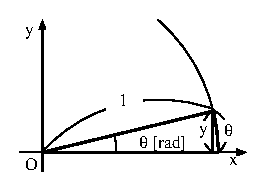
\includegraphics{small-sin.eps}}
%\begin{overpic}[width=4cm,grid,tics=10]{mapping.eps}
\begin{overpic}[width=4cm]{mapping.eps}
\put(44,68){\Large $A$}
\put(1,63){\Large $\vect{x}$}
\put(94,64){\Large $\vect{y}$}
\put(7,33){\Large ${P^{-1}}$}
\put(100,33){\Large ${P}$}
\put(45,7){\Large $\Lambda$}
\put(1,2){\Large$\hat{\vect{x}}$}
\put(94,2){\Large$\hat{\vect{y}}$}
% \put(0,-5){\small 固有ベクトル方向への拡大縮小}
\end{overpic} 
\caption{行列$A$=$P^{-1}\Lambda P$による一次変換}
\label{fig:mapping}
\end{center}
\end{figure}
さて、$A$による一次変換は次式のように書くこともできる(図\ref{fig:mapping})。
\begin{align}
  \label{eq:A=PLP}
  A\vect{x}=P\Lambda P^{-1}\vect{x}
\end{align}
この式は$A$による一次変換を以下のように分解
できることを示している。
\begin{enumerate}
\item $\vect{x}$を,固有ベクトルにそって座標軸をとった座標系に変換する
  ($P^{-1}\vect{x}$)
\item 各固有ベクトル方向に拡大する($\Lambda P^{-1}\vect{x}$)
\item もとの座標系に戻す($P\Lambda P^{-1}\vect{x}=A\vect{x}$)
\end{enumerate}

\nquestion
行列$A$,$B$が, 固有ベクトルにそった拡大縮小を決める共通の対角行列
$\Lambda$を持つとき,すなわち
\begin{align}
  A&=P\Lambda P^{-1}\notag\\
  B&=Q\Lambda Q^{-1}\notag
\end{align}
が成り立つとき,$A$と$B$は互いに\bfindex[そうじ]{相似}
(\nmindex{similar})、もしくは\bfindex[どうち]{同値}
(\nmindex{equivalent})であるという。
相似な$A$, $B$に対して以下を満たす行列$R$が存在することを示しなさい。
\begin{align}
  B=RA R^{-1}\notag
\end{align}

\nquestion
$A=P\Lambda P^{-1}$のとき以下が成り立つことを証明しなさい。
\begin{align}
  \det A=\det (P\Lambda P^{-1})
\end{align}
% \nquestion
% 式(\ref{eq:diagonalization})を利用して以下を証明しなさい。
% \begin{align}
%   \tr A=\sum_{i=0}^n\lambda_i
%\end{align}

\exercise
次のような行列$P$, $Q$, $R$について以下の問に答えなさい。
\begin{align}
P=&\begin{pmatrix} 2 & 1\\1 & 2
  \end{pmatrix},
\quad 
Q=\begin{pmatrix} -1 & 0\\1 & -2
  \end{pmatrix}
\notag\\
&R=\begin{pmatrix} 2 & -2 & 2\\1 & 1 & 0\\1 & 3 & -2
  \end{pmatrix}\notag
\end{align}
\begin{enumerate}
\item 各行列の対角化を行いなさい($P$,$R$の固有値,固有ベクトルは
  問\ref{sec:eigen}ですでに求めているはずである)。
\item $P$および$Q$はどのような一次変換を与えるか、幾何学的に説明せよ。
\item 行列$A$が与える漸化式$\vect{x_{n+1}}=A\vect{x_{n}}$を考える。
  \begin{enumerate}
  \item 行列$P$,$Q$,$R$の与える漸化式の一般解を求めなさい。
  \item 漸化式にしたがってあるベクトル$x$が繰り返し射影されるとき,
  $n\to\infty$において$x$はどのような値になるだろうか。
  その値を各行列の固有値に基づいて説明できることを示しなさい。
  \end{enumerate}
\end{enumerate}

% \subsection{行列の対角化と座標変換(old)}

% 式(\ref{eq:AP=Pl})は,行列$A$が固有ベクトルを変換する時には、そ
% の向きを変えずに大きさのみを変えることを意味する。
% またこの式より,行列$A$は以下のように書けることがわかる。
% \begin{align}
%   A=P\Lambda P^{-1}
% \end{align}
% よってあるベクトル$\vect{x}$の$A$による変換は次式のように書ける。
% \begin{align}
%   \label{eq:A=PLP}
%   A\vect{x}=P\Lambda P^{-1}\vect{x}
% \end{align}
% この式の幾何学的意味を次の設問で考えてみよう。

% \nquestion
% 座標軸の向きを表すベクトル(例えば$(1,0,0,...)$等)は
% 行列$A$による変換によって多くの場合向きを変えてしまう。
% しかし,固有ベクトルはその向きを変えないので,
% 固有ベクトルにそって座標軸をとり直すと、$A$による変換がどのようなもの
% かわかりやすそうである。
% この新しい座標軸による座標表現を$\hat{\vect{x}}$,もとの座標表現を
% $\vect{x}$とおくと,以下のような関係がある。
% \begin{align}
%   \vect{p}_1\;&\to\;   \hat{\vect{p}}_1=(1,0,0,\cdots,0)\notag\\
%   \vect{p}_2\;&\to\;   \hat{\vect{p}}_2=(0,1,0,\cdots,0)\notag\\
%   \vdots\;&\to\qquad \vdots\notag\\
%   \vect{p}_n\;&\to   \hat{\vect{p}}_n=(0,\cdots,0,1)\notag\\
%   \vect{x}=c_1\vect{p}_1+c_2\vect{p}_2+\cdots  
%   \;&\to\; \hat{\vect{x}}=c_1\hat{\vect{p}}_1+c_2\hat{\vect{p}}_2+\cdots\notag
% \end{align}
% $\hat{\vect{x}}$から$\vect{x}$に変換する行列は$P$であること,すなわち
% \begin{align}
%   \vect{x}=P\hat{\vect{x}}\notag
% \end{align}
% であることを示しなさい。

% \comment
% 上式より
% \begin{align}
%   \hat{\vect{x}}=P^{-1}\vect{x}\notag
% \end{align}
% である。
% よって式(\ref{eq:A=PLP})は$A$による一次変換を以下のように分解
% できることを示している。
% \begin{enumerate}
% \item $\vect{x}$を,固有ベクトルにそって座標軸をとった座標系に変換する
%   ($P^{-1}\vect{x}$)
% \item 各固有ベクトル方向に拡大する($\Lambda P^{-1}\vect{x}$)
% \item もとの座標系に戻す($P\Lambda P^{-1}\vect{x}=A\vect{x}$)
% \end{enumerate}
% 

\subsection{行列の標準形\prog}

任意の二次正方行列$A$は,ある行列$P$を用いた変換
$P^{-1}AP$によって,以下のいずれかの形に変換することができる。
\begin{align}
\mbox{(i)}
  \begin{pmatrix}
    \lambda_1 & 0 \\
    0 &\lambda_2
  \end{pmatrix}
\quad\mbox{(ii)}
  \begin{pmatrix}
    \alpha & \omega \\
    -\omega &\alpha
  \end{pmatrix}
\quad\mbox{(iii)}
  \begin{pmatrix}
    \lambda & 1 \\
    0 &\lambda
  \end{pmatrix}\notag
\end{align}
これらを二次正方行列の\bfindex[ひょうじゅんけい]{標準形}
(\nmindex{normal form})とよぶ。

行列$A$が一次独立な2つの固有ベクトル
をもつときには(i)の形に
変換できることは\ref{sec:diagonalization}節で既に述べた通りである。

\nquestion
二次実正方行列$A$が複素固有値$\lambda_{\pm}=\alpha\pm i\omega$,
$(\alpha,\omega\in\Real)$を持つときには(i)の形式に変換することができる。
さらに,実数行列である上記(ii)の形にも変換できることを示しなさい。\\
ヒント)$\lambda_{\pm}$に対する固有ベクトルを
$\vect{u}_{\pm}=u\pm iv$, $(u,v\in \Real)$とおき,
$A\vect{u}_+=\lambda_+\vect{u}_+$を実部と虚部に分けた連立方程式にする
と見通しがよくなる。

\nquestion
行列$A$が重複した1つの固有値$\lambda$を持つ場合を考えてみよう。
$A$が一次独立な2つの固有ベクトルをもつ場合には,既に述べたように
(i)の形式に変換できる。
一方,一次独立な固有ベクトルを1つのみもつ場合には(iii)の形式に変換で
きることを以下のように示すことができる。

固有ベクトルを$\vect{p}$とおくと,$\vect{p}$と一次独立なベクトル
$\vect{q}$に対して
\begin{align}
  \label{eq:toJordan}
  A\vect{q}=c\vect{p}+d\vect{q}
\end{align}
なる定数$c$, $d$が存在する。

\begin{enumerate}
\item この$c$, $d$が以下のように与えられることを示しなさい。
  \begin{enumerate}
  \item $c\ne 0$
  \item $d=\lambda$\\
    ヒント) $d\ne\lambda$とすると次式が成り立ち,$d\ne \lambda$なる固有値
    が存在することになるので, 題意に矛盾することを示す。
    \begin{align}
      A\left(\vect{q}+\frac{c}{d-\lambda}\vect{p}\right)
      =d\left(\vect{q}+\frac{c}{d-\lambda}\vect{p}\right)\notag
    \end{align}
  \end{enumerate}
\item 式(\ref{eq:toJordan})において$\vect{r}=\frac{1}{c}\vect{q}$とお
  くと次式が成り立つ。
  \begin{align}
    \begin{cases}
      A\vect{r}&=\vect{p}+\lambda\vect{r}\\
      A\vect{p}&=\lambda\vect{p}
    \end{cases}\notag
  \end{align}
  このことを利用してある行列$P$によって$A$を標準系(iii)に変換できるこ
  とを示しなさい。
\end{enumerate}

\nquestion
各標準形によって$\vect{x}=x(1,0)^T+y(0,1)^T$がどのような
ベクトルに写像されるかを考察することにより,
各標準形がどのような一次変換を与えるかを幾何学的に説明しなさい。


\exercise
以下の行列を標準系にしなさい。
\begin{enumerate}
\item $
  \begin{pmatrix}
    0 & 1 \\
    -4 & 0
  \end{pmatrix}
$
\item  $
  \begin{pmatrix}
    1 & 1 \\
    -1 & 3
  \end{pmatrix}
$
\end{enumerate}

\subsection{二次形式\label{sec:rotate}}
\question
以下の方程式をみたす曲線がどのような形をしているかを考えてみよう。
\begin{align}
  \label{eq:matrix-oval}
  5x^2 + 6 xy + 5y^2=8
\end{align}
この式は次のように書くこともできる。
\begin{align}
  \label{eq:quadratic-oval}
  &\vect{x}^TA\vect{x}=8,\\
  A=&
  \begin{bmatrix}
    5 & 3 \\
    3 & 5 
  \end{bmatrix},\quad
  \vect{x}={(x,y)^T}
  \notag
\end{align}
このように二次の多項式を行列を用いて表したものを
\bfindex[にじけいしき]{二次形式}(\nmindex{quadratic form})という。
\begin{enumerate}
\item 行列$A$の固有値$\lambda_1,\lambda_2$と、
  対応する固有ベクトル$\vect{p}_1,\vect{p}_2$を求めなさい。
  固有ベクトルはノルムが1になるように選びなさい。
\item 行列$A$を対角化するベクトルを$P$とする。
  座標変換$\vect{x}=P\hat{\vect{x}}$を行う。
  $P$はどのような変換を行う行列か、その幾何学的意味を説明しなさい。
\item 前問の座標変換によって、
  式(\ref{eq:quadratic-oval})を変換した方程式
  \begin{align}
    \hat{\vect{x}}^T\Lambda\hat{\vect{x}}=8,\quad 
    \Lambda=\diag\{\lambda_1,\lambda_2\}
  \end{align}
  はどのような形をした曲線か図示して説明しなさい。
\item 
  以上の結果より、式(\ref{eq:matrix-oval})は楕円を表していることを説明
  しなさい。
  特に、行列$A$の固有ベクトルが上式で表される楕円の主軸の向きを,
  また,2つの固有値の比率の平方根が,対応する固有ベクトルの表す軸の長さ
  の比率になっていることに注目し、その理由を座標変換の幾何学的意味を
  考えて説明しなさい。
\end{enumerate}

% \subsection{二次形式(old)\label{sec:rotate}}
% \question
% \begin{enumerate}
% \item  以下の方程式をみたす曲線上の各点を,
%   原点に関して時計回りに角度$\pi/4$ラジアン回転した後,
%   $x$座標のみを2倍して得られる点の集合はどのような方程式をみたすか?
%   \begin{align}
%     \label{eq:matrix-oval}
%     5x^2 + 6 xy + 5y^2=8
%   \end{align}
%   [ヒント]
%   逆行列の計算が必要な場合には,各行列の変換の意味を考え,また,式
%   (\ref{eq:PQ-1})を必要に応じて利用すると比較的簡単に計算できる。
% \item 
%   前問の結果を用いて式(\ref{eq:matrix-oval})のグラフを描きなさい。
% \item 
%   前問の結果により式(\ref{eq:matrix-oval})は楕円を表すことがわかる。
%   この式は次のように書くこともできる。
%   \begin{align}
%     \vect{x}^TA\vect{x}=8,\quad 
%     A=
%     \begin{bmatrix}
%       5 & 3 \\
%       3 & 5 
%     \end{bmatrix},\quad
%     \vect{x}={(x,y)^T}
%     \notag
%   \end{align}
%   このように二次の多項式を行列を用いて表したものを
%   \bfindex[にじけいしき]{二次形式}(\nmindex{quadratic form})という。

%   行列$A$の固有ベクトルが上式で表される楕円の主軸の向きを,
%   また,2つの固有値の比率の平方根が,対応する固有ベクトルの表す軸の長さ
%   の比率になっていることを確認せよ。
% \end{enumerate}

\subsection{微分方程式の行列を用いた解法}
微分方程式
\begin{align}
  \label{eq:diff-matrix}
  \ddot{x}+3\dot{x}+2x=0
\end{align}
について以下の問に答えなさい。
\begin{enumerate}
\item $\dot{x}=y$とおくと,式(\ref{eq:diff-matrix})を以下のように書け
  ることを示しなさい。
  \begin{align}
    \label{eq:matrix}
    &\dot{\boldsymbol{x}}=A\boldsymbol{x}\\
    \boldsymbol{x}=
    \begin{pmatrix}
      x \\ y
    \end{pmatrix}_,& \quad
    A= \begin{pmatrix}
      0 & 1 \\
      -2 & -3
    \end{pmatrix}_.\notag
  \end{align}
\item 行列Aの固有値と固有ベクトルを求めなさい。
\item 行列Aを対角化する行列Pを求めなさい。
\item 
  座標変換$\vect{x}=P\hat{\vect{x}}$を利用して微分方程式
  (\ref{eq:matrix})を以下の形に変形しなさい。
  \begin{align}
    \dot{\hat{\vect{x}}}=\Lambda\hat{\vect{x}},\quad
    \Lambda=P^{-1}AP\notag
  \end{align}
  上式より解$\hat{\vect{x}}$は容易に求まる。
  その結果を利用して解$\boldsymbol{x}$を求めなさい。
\end{enumerate}

%% \section{3次元空間内の回転}
%% 3次元空間内の点$P$の位置を,位置ベクトル$\boldsymbol{p}=(x,y,z)^T$で表す。
%%   \begin{enumerate}
%%   \item 点$P$を$x$軸のまわりに,角度$\theta$だけ回転する行列を$R_x(\theta)$求めよ。
%%     右ネジが$x$軸方向に進むときの回転方向を正とする。
%%   \item  点$P$を$y$軸のまわりに,角度$\theta$だけ回転する行列を$R_y(\phi)$求めよ。
%%   \item  点$P$を$z$軸のまわりに,角度$\theta$だけ回転する行列を
%%     $R_z(\psi)$求めよ。
%%   \item 回転変換においては,交換則はなりたたない。そのことを説明せよ。
%%   \end{enumerate}

\newpage% 


\appendix
\section{TODO}
西井用のメモコーナーです。見ないで下さい\verb|(^^);;|
\begin{enumerate}
\item 対角化の問題を充実
  \begin{enumerate}
  \item 対称行列の対角化
  \item 固有値が複素数になる場合
  \item 固有値が縮退する場合
  \item Jordan標準形
  \end{enumerate}
\end{enumerate}% 

\section{このドキュメントの著作権について}

\begin{enumerate}
\item 本稿の著作権は西井淳\url{nishii@sci.yamaguchi-u.ac.jp}が有します。
\item 非商用目的での複製は許可しますが,修正を加えた場合は必ず修正点および加筆者の
氏名・連絡先,修正した日付を明記してください。また本著作権表示の削除は行っ
てはいけません。
\item 本稿に含まれている間違い等によりなんらかの被害を被ったとしても著者は一切
責任を負いません。
\end{enumerate}
間違い等の連絡や加筆修正要望等の連絡は大歓迎です。

%% \newpage
%% \section{在庫中の問題}
%% \section{全微分}

%% おもりを糸で吊したとき,おもりが重力で揺れる周期$T$は,
%% その糸の長さを$l$とすると
%% \begin{align}
%%   T=2\pi\sqrt{\frac{l}{g}}\notag
%% \end{align}
%% で表される。ここで$g$は重力の大きさを表す定数(重力加速度の大きさ)である。
%% 糸の長さ$l$と重力加速度の大きさ$g$がそれぞれ微小量$dl$,
%% $dg$変化した時の周期$T$の変化の割合$dT/T$を求めよ。($T$の全微分を求めればよい)。

\printindex% 

\end{document}
